% Compilar usando LuaLaTeX.

\documentclass{book}

% Configuraciones:

% O comando abaixo pode ser necessário em documentos que usam versões antigas do pacote "fontspec". Se for começar um novo documento, deixe esse linha comentada e use caracteres Unicode.
% \usepackage[utf8]{luainputenc}


% Licencia CC
\usepackage[
    type={CC},
    modifier={by-sa},
    version={3.0},
    lang={sp},
]{doclicense}
% Tamanho do papel e das margens: 
\usepackage{rotating}
\usepackage[paperheight=230mm,paperwidth=160mm,inner=20mm,outer=14mm,top=24.5mm,bottom=21mm,pdftex]{geometry}

% Suporte a idiomas:

\usepackage[greek,brazilian,spanish]{babel}

% Para usar as variáveis \theauthor, \thetitle e \thedate (autor, título e data).

\usepackage{titling}

% Título de capítulo elegante:

\usepackage[Lenny]{fncychap}

% Pacote para estilo elegante:

\usepackage{fancyhdr}

% Definição de novas cores:

\usepackage{xcolor}

\definecolor{verde}{rgb}{0.2, 0.50, 0.25}
\definecolor{verde_UnB}{cmyk}{1,0,1,0.4}
\definecolor{cinza_UnB}{rgb}{0.6,0.6,0.6} % https://www.ginifab.com/feeds/pms/color_picker_from_image.php


% Para mudar cor de títulos (https://tex.stackexchange.com/a/75670/91816):

\usepackage{sectsty}

\chapterfont{\color{verde_UnB}}  % sets colour of chapters
\sectionfont{\color{verde_UnB}}  % sets colour of sections

% Pacote para definir fonte de qualquer tamanho:

\usepackage{fix-cm}

%% Pacote para correta separação silábica de palavras com hífen;
%% hífens devem ser escritos como \Hyphdash ou \-/ (se opção shortcuts estiver ativa)
%% no texto; por exemplo cana\-/de\-/açúcar seria separada como
%% cana-de- numa linha e -açúcar na linha seguinte
%% repetindo o hífen (um hífen é da separação e outro é da palavra):

\usepackage[shortcuts]{extdash}

%% Definindo espacamento:

\usepackage{setspace} 
\singlespacing

%% Enumerar itens:

\usepackage{enumitem}

%% Pacote para criar caixas:

\usepackage{pbox} %  que limitam a largura de textos em células,
%\usepackage{minibox} % que têm largura arbitrária.

%% Definição das dimensões do texto:

%\setlength{\textwidth}{16cm}
%\setlength{\textheight}{22cm}
%\setlength{\headheight}{1cm}
%\setlength{\footheight}{1cm}

\usepackage[title,titletoc]{appendix}

%% Passando títulos para o português:

\renewcommand{\chaptername}{Capítulo}
\renewcommand{\bibname}{Referencias}
\renewcommand{\appendixname}{Anexo}
\renewcommand{\indexname}{Índice}
\renewcommand{\contentsname}{\bf\color{verde_UnB}Contenidos}
\renewcommand{\tablename}{Tabla}
\renewcommand{\figurename}{\bf Fig.}
\renewcommand{\sin}{sen}
\def\listoffiguresname{Lista de Figuras}
\def\listoftablesname{Lista de Tablas}

%% Definindo estilo de pagina:

\pagestyle{fancy}

% PACOTES DE TABELAS:

%% Espaçamento de tabelas ajustado:

\usepackage{booktabs}

%% Pacotes de linhas e colunas multiplas:

\usepackage{multirow}
\usepackage{multicol}

%% Pacotes de tabela e tabulação:

%%% Tabela com caixas centralizada:

\usepackage{array}
\newcolumntype{P}[1]{>{\centering\arraybackslash}p{#1}}

%%% Tabela em múltiplas páginas:

\usepackage{longtable}

%%% Tabela colorida:

\usepackage{tabu}
\usepackage{colortbl}

%%% Mudando cor das linhas de todas as tabelas:

\makeatletter
\renewenvironment{table}
     {\@float{table}\taburulecolor{verde_UnB}\arrayrulecolor{verde_UnB}}
     {\end@float}
\makeatother

%%% Tabela com linhas pontilhadas:

\usepackage{arydshln}

% PACOTES MATEMÁTICOS:

%% Pacote para não-itálico em ambiente de fórmulas:
%\usepackage[]{mathastext}

%% Pacotes matemáticos:

\usepackage{amsmath}
\usepackage{mathtools}

%%% Numera apenas equações usadas:

%\mathtoolsset{showonlyrefs=true}

%%% Declarando barras para valor absoluto e norma:

\DeclarePairedDelimiter\abs{\lvert}{\rvert}%
\DeclarePairedDelimiter\norm{\lVert}{\rVert}%

%% Nome de equações ao lado com comando "eqname":

\newcommand{\eqname}[1]{\tag*{\llap{#1}}}

%% Fontes tipográficas:

\usepackage{fontspec}
%\usepackage{libertineotf}

%%% Seleção da fonte UnB Pro:

\setmainfont{UnB-Pro}[
  Path = fonts/UnB_Pro_v1.0/,
  Extension=.otf,
  UprightFont=*_Regular,
  ItalicFont=*_Italic,
  BoldFont=*_Bold,
  BoldItalicFont=*_Bold-Italic,
]

\setmonofont{Libertinus Mono}

%%% Para incluir o comando \url{}:

\usepackage[breaklinks=true, hidelinks]{hyperref}

%% Configurações ABNTeX:

\usepackage[hyphens,alf,abnt-and-type=e,abnt-last-names=bibtex,abnt-etal-cite=1,abnt-etal-list=1]{abntex2cite}


% Recuo no primeiro parágrafo:

\usepackage{indentfirst}

% Mudando recuo de parágrafo e tamanho da fonte:

\setlength{\parindent}{7mm}
\fontsize{11pt}{13.2pt}\selectfont

% Usado para evitar linhas órfãs:

\usepackage{needspace}

% Mudar espaçamento entre número e título de seção:

%% \def\l@figure{\@dottedtocline{1}{1.5em}{2.5em}}

\usepackage{tocloft}
\setlength{\cftfignumwidth}{2.55em} 

% Para escrever "Apêndices" e "Anexos":

%\usepackage[titletoc]{appendix}

% Elimina recuo nas notas de rodapé:

\usepackage[hang,flushmargin]{footmisc}

% Primeira página vazia em cada capítulo:

\makeatletter
\renewcommand\chapter{\if@openright\cleardoublepage\else\clearpage\fi
                    \thispagestyle{empty}% original style: plain
                    \global\@topnum\z@
                    \@afterindentfalse
                    \secdef\@chapter\@schapter}
\makeatother

% Diminui chance de linhas órfãs e viúvas:

\clubpenalty1000000
\widowpenalty1000000

% Comando para mudar a fonte de citação literal de código (verbatim):

\makeatletter
\newcommand{\verbatimfont}[1]{\def\verbatim@font{#1}}%
\makeatother

% Pacote para referir a capítulos pelo nome:
\usepackage{nameref}
\makeatletter
\newcommand*{\currentname}{\@currentlabelname}
\makeatother

% Definições (alternativas a nameref) para se referir a capítulos e seções pelo nome:
\let\Chaptermark\chaptermark
\def\chaptermark#1{\def\Chaptername{#1}\Chaptermark{#1}}
\let\Sectionmark\sectionmark
\def\sectionmark#1{\def\Sectionname{#1}\Sectionmark{#1}}
\let\Subsectionmark\subsectionmark
\def\subsectionmark#1{\def\Subsectionname{#1}\Subsectionmark{#1}}
\let\Subsubsectionmark\subsubsectionmark
\def\subsubsectionmark#1{\def\Subsubsectionname{#1}\Subsubsectionmark{#1}}

% Pacote para usar "clearpage" sem finalizar página, apenas descarregar todos os elementos já inseridos:

\usepackage{afterpage}

% Pacote para que páginas em branco não mostrem cabeçalhos nem rodapés:

\usepackage{emptypage}

% Pacote para índice Remissivo (a ser impresso por \printindex):

\usepackage{makeidx}
\makeindex

% Pacotes auxiliares no design da capa:

% Códigos QR
\usepackage{qrcode}

%Por defecto:\quad
%\qrcode{https://www.jmmaffei.com}
%\qquad

%+1" de alto y de largo:
%\quad
%\qrcode[height=1in]{https://www.ctan.org/tex-archive/macros/latex/contrib/qrcode?lang=en}

\usepackage{xcoffins}
%\usepackage{svg}
%% Pacotes para usar o pacote Metapost para fazer graficos e diagramas:

\usepackage{luamplib}
\everymplib{input mpcolornames; beginfig(1);}
\everyendmplib{endfig;}
% Paquete para imágenes Postscript
%\usepackage{epsf} 
%% Pacotes para diagramas, desenhos, gráficos:


\usepackage{tikz}
\usetikzlibrary{backgrounds,patterns}

\usepackage{pgfplots}
\pgfplotsset{compat=1.12}

%% Pacote para ferramentas gráficas:

\usepackage{graphics}
\usepackage{graphicx} % Sem esse, alguns includegraphics não funcionam.


\usepackage[pdf]{pstricks}
\usepackage{pst-node,pst-circ,pst-plot,pst-3dplot,pst-all}

\usepackage{threeparttable} % Para alinhar figuras e legendas com "measuredfigure".

\usepackage{wrapfig} % Figuras ao lado do texto.

\usepackage{picinpar}% Alteranativa para figuras ao lado de texto. http://ctan.org/pkg/picinpar

\usepackage[font={small}, margin=0cm, justification=centering]{caption} % Legendas com fonte pequena.

% Comando para adicionar fonte de figuras e semelhantes:

\newcommand{\source}[1]{\captionsetup{singlelinecheck=false,justification=justified}\caption*{\footnotesize \noindent Fonte: {#1}}}
% Tamanhos de fontes matemáticas em relação à fonte do texto:
%% {tamanho do texto} {matemática} {matemática script} {matemática scriptscript}

\DeclareMathSizes{10}{10}{6}{4}
\DeclareMathSizes{9}{9}{5}{3}

\usepackage{amsthm} % deve ser chamado antes de mdframed conforme dito em http://tex.stackexchange.com/questions/283763/why-dont-i-get-non-italic-normal-font-inside-theorem-environment-using-newmdth

% Seleção de fontes de equações:

\usepackage[math-style=french]{unicode-math} % não funciona se compilar com pdflatex, deve-se usar xelatex ou lualatex

\usepackage{yfonts} % para usar caracteres góticos para algumas variaveis

% Pacote para maior controle de fluxo de figuras (usado para opção [H] que fixa a posição das figuras):

\usepackage{float}

% Pacote usado para impedir elementos flutuantes (figuras, tabelas, etc.) de aparecerem em seção errada:

\usepackage[section]{placeins}

% Pacote inserido para fazer o símbolo de grau:

\usepackage{gensymb}

% Pacote inserido para fazer símbolos de circuito elétrico:

\usepackage{marvosym}

% Definição de variáveis e unidades:

\newcommand{\angstrom}{\text{\normalfont\AA}}
\newcommand{\pol}{\ensuremath{pol}}
\newcommand{\cm}{\ensuremath{cm}}
\newcommand{\km}{\ensuremath{km}}
\newcommand{\hm}{\ensuremath{hm}}
\newcommand{\dam}{\ensuremath{dam}}
\newcommand{\dm}{\ensuremath{dm}}
\newcommand{\mol}{\ensuremath{mol}}
\newcommand{\mi}{\ensuremath{mi}}
\newcommand{\h}{\ensuremath{h}}
\newcommand{\s}{\ensuremath{s}}
\newcommand{\Min}{\ensuremath{min}}
\newcommand{\Pa}{\ensuremath{Pa}}
\newcommand{\atm}{\ensuremath{atm}}
\newcommand{\mmHg}{\ensuremath{mmHg}}
\newcommand{\BarP}{\ensuremath{Bar}}
\newcommand{\PsiP}{\ensuremath{PSI}}
\newcommand{\lb}{\ensuremath{lb}}
\newcommand{\N}{\ensuremath{N}}
\newcommand{\kg}{\ensuremath{kg}}
\newcommand{\kgf}{\ensuremath{kgf}}
\newcommand{\are}{\ensuremath{a}}
\newcommand{\litro}{\ensuremath{\ell}}
\newcommand{\g}{\ensuremath{g}}

% Símbolos de diferencial:

\def\D{\mathrm{d}} %% diferencial - comando \D{}
\def\DI{{\delta}} % diferencial inexata ``delta''

\newcommand*\diff{\mathop{}\!\mathrm{d}}
\newcommand*\Diff[1]{\mathop{}\!\mathrm{d^#1}}

% Evita que equações extrapolem a margem (e permite outros recursos tipográficos avançados):

\usepackage{microtype}

%% Simbolos matemáticos extra:

\DeclareMathSymbol{\Omega}{\mathalpha}{letters}{"0A}
\DeclareMathSymbol{\varOmega}{\mathalpha}{operators}{"0A}
\providecommand*{\upOmega}{\varOmega} % for siunitx

%% Pacote para uso de unidades SI com distância padronizada entre valor e unidade:

\usepackage{siunitx}
\sisetup{%
      binary-units=true,
      group-separator={.},
      group-digits=integer,
      load-configurations=abbreviations,
      load=addn,
      per-mode=fraction,
      output-decimal-marker={,},
      range-phrase= --,
      separate-uncertainty=true,
      math-ohm = \ensuremath{\upOmega}, % senão \ohm não funciona
      text-ohm = Ω,  % senão \ohm não funciona
    }

\DeclareSIUnit\milha{mi}
\DeclareSIUnit\polegada{pol}
\DeclareSIUnit\alqueire{alqueire}
\DeclareSIUnit\inch{in}
\DeclareSIUnit\foot{ft}
\DeclareSIUnit\kgf{kgf}
\DeclareSIUnit\lbf{lbf}
\DeclareSIUnit\pound{lb}
\DeclareSIUnit\rev{rev}
\DeclareSIUnit\rpm{rpm}
\DeclareSIUnit\pkt{PKT}
\DeclareSIUnit{\calorie}{cal}
\DeclareSIUnit{\cal}{cal}
\DeclareSIUnit{\Cal}{Cal}
\DeclareSIUnit{\Calorie}{\kilo\calorie}
\DeclareSIUnit{\fahrenheit}{\degree F}

\DeclareSIUnit{\nothing}{\relax} % usado para mostrar prefixos sem unidade

% Definição de ambientes exercício, solução, definição, exemplo, demonstração, etc.

\usepackage{mdframed}

\usepackage{environ} % usado nas definições \MakeDiscussionTopSecret, \MakeDiscussionsPublic, etc.

% Exercício e solução (pacote Exsheets):

\usepackage{exsheets} %[2015/02/09]

% Configurações do pacote Exsheets:

\SetupExSheets{
  headings          = block-subtitle ,
  subtitle-format   = \sc ,
  counter-within    = {chapter} , % Contar dentro dos capítulos.
  counter-format    = ch.qu[1] , % Formato 1.1, 1.2, 1.3, etc.
  label-format      = ch.qu[1] , % Formato 1.1, 1.2, 1.3, etc.
  headings-format   = \bfseries ,
  question/pre-hook = \needspace{0.3\textheight}\vspace{1ex} ,
  question/post-hook = \vspace{1ex} ,
  question/pre-body-hook = {\vspace{1ex} \mdframed[backgroundcolor=verde_UnB!10, linewidth=1pt, innermargin=+0cm, outermargin=+0cm]},
  question/post-body-hook = \endmdframed ,
  solution/pre-hook = \needspace{0.3\textheight}\vspace{1ex},
  solution/post-hook = \vspace{1ex},
  solution/pre-body-hook = \vspace{1ex},
  solution/print    = false
}

\renewcommand\thequestion{\thechapter.\arabic{question}} % Formato 1.1, 1.2, 1.3, etc., ao usar \ref{}:

% Ambiente "Ejemplo":

\mdfdefinestyle{definitionSty}{backgroundcolor=gray!10, linecolor=verde_UnB, linewidth=0pt, innerleftmargin=3ex, innerrightmargin=3ex, innertopmargin=1ex, innerbottommargin=1ex, innermargin =0, outermargin =0, needspace={0.2\textheight}}
\newcounter{definitionCounter}[chapter]
\numberwithin{definitionCounter}{chapter}
\theoremstyle{definition}
\newmdtheoremenv[style=definitionSty]{ejemplo}[definitionCounter]{Ejemplo}

% Ambiente "Teorema":

\mdfdefinestyle{theoremSty}{backgroundcolor=verde_UnB!10, linecolor=verde_UnB, linewidth=0pt, innerleftmargin=3ex, innerrightmargin=3ex, innertopmargin=1ex, innerbottommargin=1ex, innermargin=0, outermargin=0, needspace={0.2\textheight}}
\newcounter{theoremCounter}[chapter] 
\numberwithin{theoremCounter}{chapter}
\newmdtheoremenv[style=theoremSty]{theorem}[theoremCounter]{Teorema}

% Ambiente "Demonstração":

\mdfdefinestyle{demonstrationSty}{backgroundcolor=gray!10, linecolor=verde_UnB, linewidth=0pt, innerleftmargin=3ex, innerrightmargin=3ex, innertopmargin=1ex, innerbottommargin=1ex, innermargin =0cm, outermargin =0cm, needspace={0.2\textheight}}
\newcounter{demonstrationCounter}[chapter]
\numberwithin{demonstrationCounter}{chapter}
\newmdtheoremenv[style=demonstrationSty]{demonstration}[demonstrationCounter]{Demonstra\c{c}\~{a}o}

% Ambiente "Axioma":

\mdfdefinestyle{axiomSty}{backgroundcolor=verde_UnB!10, linecolor=verde_UnB, linewidth=1pt, innerleftmargin=3ex, innerrightmargin=3ex, innertopmargin=1ex, innerbottommargin=1ex, innermargin=0, outermargin=0, needspace={0.1\textheight}}
\newcounter{axiomCounter}[chapter] 
\numberwithin{axiomCounter}{chapter}
\newmdtheoremenv[style=axiomSty]{axiom}[axiomCounter]{Axioma}

% Ambiente "Exemplo":

\mdfdefinestyle{exampleSty}{backgroundcolor=gray!10, linecolor=verde_UnB, linewidth=0pt, innerleftmargin=3ex, innerrightmargin=3ex, innertopmargin=1ex, innerbottommargin=1ex,  innermargin =+0cm, outermargin =+0cm, needspace={0.2\textheight}}
\newcounter{exampleCounter}[chapter]
\numberwithin{exampleCounter}{chapter}
\newmdtheoremenv[style=exampleSty]{example}[exampleCounter]{Exemplo}

% Ambiente "Problema":

\mdfdefinestyle{problemSty}{backgroundcolor=gray!10, linecolor=black, linewidth=1pt, innerleftmargin=3ex, innerrightmargin=3ex, innertopmargin=1ex, innerbottommargin=1ex, innermargin =+0cm, outermargin =+0cm, needspace={0.15\textheight}}
\newcounter{problemCounter}[chapter]
\numberwithin{problemCounter}{chapter}
\newmdtheoremenv[style=problemSty]{problem}[problemCounter]{Problema}

% Ambiente "Nota":

\mdfdefinestyle{noteSty}{backgroundcolor=white, font=\small, fontcolor=verde_UnB, linecolor=verde_UnB, linewidth=1pt, innerleftmargin=3ex, innerrightmargin=3ex, innertopmargin=2ex, innerbottommargin=2ex, innermargin =+0cm, outermargin =+0cm, needspace={0.1\textheight}}
\newcounter{noteCounter}[chapter]
\numberwithin{noteCounter}{chapter}
\newmdtheoremenv[style=noteSty]{note}[noteCounter]{Nota}

% Ambiente "Discussão" (texto complementar):

\mdfdefinestyle{discussionSty}{backgroundcolor=white, fontcolor=verde_UnB, linecolor=verde_UnB, linewidth=0pt, innerleftmargin=3ex, innerrightmargin=3ex, innertopmargin=3ex, innerbottommargin=3ex, innermargin=+0cm, outermargin =+0cm, needspace={0.25\textheight}}
\newcounter{discussionCounter}%[chapter]
%\numberwithin{discussionCounter}{chapter}
\newmdtheoremenv[style=discussionSty]{discussion}[discussionCounter]{Texto Complementar}

% Ambiente "Dedicatória" (baseado em https://tex.stackexchange.com/a/167529/91816):

\newenvironment{dedication}
  {
    \itshape             % the text is in italics
    \raggedleft          % flush to the right margin
  }
  {
    \par % end the paragraph
  }
  % space at bottom is three times that at the top
  
% Citação com autor:

\renewenvironment{quotation}
  {\small\list{}{\rightmargin=0.1cm \leftmargin=4cm \topsep=1.5\baselineskip}%
   \item\relax}
  {\endlist}

\def\signed #1{{\leavevmode\unskip\nobreak\newline
  \hbox{}\nobreak #1 %
  \hfil\parfillskip=0pt \finalhyphendemerits=0 \endgraf}}

\newsavebox\mybox
\newenvironment{citacao}[1]
  {\savebox\mybox{#1}\begin{quotation}}
  {\signed{\usebox\mybox}\end{quotation}}


\title{Introducción a las mediciones eléctricas \\ EETP 669}
\author{Prof. Juan Manuel Maffei} % Para mais de um autor, use: \author{autor1 \\ autor2 \\ autor3}
\date{Abril de 2019}

% Encabezado de páginas impares (odd), izquierda (LO), centro (CO) y derecha (RO):

\makeatletter
\fancyhead[LO]{}
\fancyhead[CO]{\small \if@mainmatter \small \leftmark \fi}
\fancyhead[RO]{}
\makeatother

% Cabeçalhos das páginas pares (even):
% Obs.: caso haja mais de um autor, substitua \theauthor pelo nome do 1º autor, e coloque os outros em CE ou RE:

\fancyhead[LE]{\theauthor}
\fancyhead[CE]{}
\fancyhead[RE]{Escuela de Educación Técnico Profesional N 669} 

% Rodapé:

\fancyfoot[C]{\small \thepage}
%\fancyfoot[RO]{\small \nouppercase \rightmark}

% Para que \mainmatter não resete a contagem de páginas (https://tex.stackexchange.com/questions/380816/prevent-frontmatter-to-reset-counting):

\makeatletter
\renewcommand\mainmatter{%
  \cleardoublepage
  \@mainmattertrue
  \renewcommand{\thepage}{\arabic{page}}
  %\pagenumbering{arabic}% Don't reset
}
\makeatother

% Início do documento:

\begin{document}

% Ajustando espaços no sumário:

\makeatletter
\renewcommand{\@pnumwidth}{2.0em}
\renewcommand{\@tocrmarg}{2.7em}
\makeatother

% Parte Pré-Textual:

\frontmatter
%\pagestyle{empty}

% O código do texto está nos arquivos dentro da pasta "txt".
% Por exemplo, o comando \thispagestyle{empty}

%%% Capa: 
%%% Modelo tirado de http://tex.stackexchange.com/questions/17579/how-can-i-design-a-book-cover

\vspace*{\fill}

\begin{center}
\textbf{\color{verde_UnB}\fontsize{38pt}{45.6pt}\selectfont \textbf{Introducción a las Mediciones Eléctricas}}
\end{center}

\vspace{4 em}
\begin{center}
	\textbf{\color{verde_UnB}\fontsize{18pt}{20pt}\selectfont
	\textbf{Escuela de Educación Técnico Profesional N 669}}
\end{center}
\vfill

\begin{center}
	\textbf{2019}
\end{center}
\vspace*{\fill}

\clearpage inclui o código que está no arquivo "titulo.tex" dentro da pasta txt.
% Crie seus próprios arquivos à vontade e inclua-os aqui com o comando \include{}.

\thispagestyle{empty}

%%% Capa: 
%%% Modelo tirado de http://tex.stackexchange.com/questions/17579/how-can-i-design-a-book-cover

\vspace*{\fill}

\begin{center}
\textbf{\color{verde_UnB}\fontsize{38pt}{45.6pt}\selectfont \textbf{Introducción a las Mediciones Eléctricas}}
\end{center}

\vspace{4 em}
\begin{center}
	\textbf{\color{verde_UnB}\fontsize{18pt}{20pt}\selectfont
	\textbf{Escuela de Educación Técnico Profesional N 669}}
\end{center}
\vfill

\begin{center}
	\textbf{2019}
\end{center}
\vspace*{\fill}

\clearpage
\clearpage

%\thispagestyle{empty}

\begin{center}

\begin{tabular}{r:l}
						& \textbf{\Large EETP N 669}				\\
						&														\\
	{\bf Autor} 		& Juan Manuel Maffei									\\
%	{\bf Vice-Reitor}	& Enrique Huelva										\\
						&														\\
						& \textbf{\Large jmmaffei.com}							\\
						&														\\
	{\bf Corrección}		& Valeria Grassini 							\\
						&														\\
	{\bf Revisión técnica}	&	nnnnnnnnnnnnn					\\
								&	nnnnnnnnnnn					\\

\end{tabular}

\end{center}



\clearpage

%\clearpage

% 1ª página de cada capítulo tem estilo "vazio" (sem cabeçalho ou rodapé):
\thispagestyle{empty}

\begin{center}

\vspace*{\fill}

\textbf{\color{verde_UnB}\fontsize{30pt}{35pt}\selectfont \textbf{Introducción a las Mediciones Eléctricas}}

\vfill

{\textbf{\fontsize{13pt}{15.6pt}\selectfont \centering  Prof. Juan Manuel Maffei}}

%\vspace{1cm}

%{\textbf{\fontsize{13pt}{15.6pt}\selectfont \centering  Nome do segundo autor}}

\vspace*{\fill}
\doclicenseThis

\end{center}
Usted es libre de:
\begin{itemize}
	\item Compartir — copiar y redistribuir el material en cualquier medio o formato
	\item Adaptar — remezclar, transformar y construir a partir del material para cualquier propósito, incluso comercialmente.
\end{itemize}

Bajo los siguientes términos:
\begin{itemize}
	\item Atribución — Usted debe dar crédito de manera adecuada, brindar un enlace a la licencia, e indicar si se han realizado cambios. Puede hacerlo en cualquier forma razonable, pero no de forma tal que sugiera que usted o su uso tienen el apoyo de la licenciante.
	\item CompartirIgual — Si remezcla, transforma o crea a partir del material, debe distribuir su contribución bajo la lamisma licencia del original.
	\item No hay restricciones adicionales — No puede aplicar términos legales ni medidas tecnológicas que restrinjan legalmente a otras a hacer cualquier uso permitido por la licencia.	
\end{itemize}

\newpage
\clearpage

%\thispagestyle{empty}

\begin{center}

\begin{tabular}{r:l}
						& \textbf{\Large Escuela de Educación Técnico Profesional N 669}				\\
						&														\\
	{\bf Revisión técnica} 		& nnnnnnnnnnnnnnnnnnn					\\
	{\bf Diseño}				& Juan Manuel Maffei				\\
						&														\\
						& \textcopyright 2019 Juan Manuel Maffei	\\
						&														\\
						& CC					\\

\end{tabular}

\end{center}

\newpage

%\clearpage

%\thispagestyle{empty}

\vspace*{\fill}

\begin{dedication}
    A minha avozinha Renilda, \\
    que me ensinou a bordar, tocar violão, \\
    cuidar de peixes de aquário, produzir licor \\
    e montar um orquidário, \\
    e de quem herdei o diletantismo.    \vspace{\baselineskip}
%    \usefont{T1}{LobsterTwo-LF}{bx}{it}
%    Leonardo
\end{dedication}

% Para inserir várias dedicatórias, descomente as duas linhas acima para colocar a assinatura do autor e use o modelo abaixo para fazer uma outra dedicatória:

%\vspace{5\baselineskip}

%\begin{dedication}
%	
%    \vspace{\baselineskip}
%    \usefont{T1}{LobsterTwo-LF}{bx}{it}
%    Autor 2
%\end{dedication}
%\cleardoublepage

%\chapter*{Agradecimentos}
\thispagestyle{empty}

\hfill %\hspace{0.5cm}

Ao Decanato de Ensino de Graduação da UnB, pelo processo de seleção de livros didáticos.

A toda a equipe da Editora UnB, pela oportunidade e pelo suporte, em especial ao revisor Tiago Rodrigues.

Ao Centro de Informática da UnB, pelo suporte tecnológico.

Ao professor Olavo Leopoldino da Silva Filho, que foi meu coautor do livro Física para Ciências Agrárias e Ambientais.

À equipe do Overleaf, em especial a Lian Tze Lim pela solução de vários problemas.

A incontáveis desenvolvedores de pacotes para TeX/LaTeX e participantes de fóruns pelos quais resolvemos vários problemas relacionados a esses sistemas de editoração.

Ao fórum TeX - LaTeX do site Stack Exchange, no qual até mesmo os próprios desenvolvedores dos pacotes frequentemente responderam às questões.
%\cleardoublepage

% Lista de símbolos/variáveis:

%\chapter*{Lista de símbolos}
\thispagestyle{empty}

\vspace{0.5cm}

\begin{longtable}{|c|l|} % "|" = "linha vertical", "c" = "centro", "l" = "esquerda", "r" = "direita"
 \hline
  \textbf{Variável} & \textbf{Grandeza representada} \\ \hline
  $A$ & área \\ \hline
  $\alpha$, $\beta$, $\gamma$ & radiações \\ \hline
  $a$ & aceleração \\ \hline
  $\mathcal{B}$ & campo magnético \\ \hline
  $D$ & diâmetro \\ \hline
  $d$ & deslocamento, distância \\ \hline
  $\textgoth{D}$ & dose absorvida \\ \hline
  $\Delta{X}$ & variação ou margem de erro da medida $X$ \\ \hline
  $\D{X}$ & elemento infinitesimal, diferencial da grandeza $X$ \\ \hline
  $\DI{X}$ & diferencial inexata da grandeza $X$ \\ \hline
  $E$ & energia \\ \hline
  $\mathcal{E}$ & campo elétrico \\ \hline
  $\epsilon$  & permissividade elétrica \\ \hline
  $\eta$ & coeficiente de viscosidade \\ \hline
  $F$ & força \\ \hline
  $\phi$   & ângulo, ângulo azimutal (coordenadas polares ou esféricas) \\ \hline
  $h$ & altura, elevação \\ \hline
  $H$ & dose equivalente \\ \hline
  $I$ & corrente elétrica \\ \hline
  $K$ & energia cinética \\ \hline
  $k$ & constante elástica \\ \hline
  $k$ & número de onda, vetor de onda ($\vec{k}$) \\ \hline
  $\kappa$ & constante eletrostática de um meio \\ \hline
  $\kappa_0$ & constante de Coulomb (constante eletrostática do vácuo) \\ \hline
  $L$ & lado \\ \hline
  $L$ & momento angular \\ \hline
  $l$ & comprimento \\ \hline
  $m$ & massa \\ \hline
  $\mu$ & permeabilidade magnética \\ \hline
  $\mu_{din}$ & coeficiente de atrito dinâmico \\ \hline
  $\mu_{est}$ & coeficiente de atrito estático \\ \hline
  $N$ & força normal \\ \hline
  $\hat{n}$ & vetor normal unitário \\ \hline
  $P$ & peso \\ \hline
  $\mathscr{P}$ & potência \\ \hline
  $p$ & momento linear \\ \hline
  $\mathscr{p}$ & pressão \\ \hline
  $Q$ & calor \\ \hline
  $\mathscr{Q}$ & vazão \\ \hline
  $\textgoth{Q}$ & fator de qualidade \\ \hline  
  $q$ & carga elétrica \\ \hline
  $r$ & coordenada radial \\ \hline
  $r$, $\theta$ & coordenadas polares \\ \hline
  $r$, $\theta$, $\phi$ & coordenadas esféricas \\ \hline  
  $R$ & raio \\ \hline
  $\mathscr{R}$ & resistência elétrica \\ \hline
  $\rho$ & densidade \\ \hline
  $T$ & temperatura \\ \hline
  $\tau$ & torque, momento de força \\ \hline
  $\omega$ & velocidade angular \\ \hline
  $\mathscr{T}$ & força de tensão \\ \hline
  $T$ & temperatura \\ \hline
  $U$ & energia potencial \\ \hline
  $\mathscr{U}$ & diferença de potencial elétrico (voltagem) \\ \hline
  $v$ & velocidade \\ \hline
  $\mathscr{W}$ & trabalho \\ \hline 
  $x$ & deformação linear \\ \hline
  $\bar{x}$ & média de x \\ \hline
  $\vec{x}$ & vetor x \\ \hline
  $\mathscr{x}$, $\mathscr{y}$, $\mathscr{z}$ & eixos de um plano cartesiano \\ \hline
  $\textgoth{X}$ & exposição \\ \hline
\end{longtable}
%\cleardoublepage

% Lista de figuras:

%\listoffigures \thispagestyle{empty}
%\cleardoublepage

% Lista de tabelas:

%\listoftables \thispagestyle{empty}
%\cleardoublepage

% Sumário:

\tableofcontents\thispagestyle{empty}
\cleardoublepage 

% Parte Textual:

\mainmatter
\chapter{Sobre las mediciones}
\section{Magnitudes}
Medir es \textbf{comparar el valor de una magnitud con otro}, al que se consideró \textbf{la unidad} de dicha magnitud, a través de un experimento físico.

Una \textbf{magnitud} es toda aquella propiedad de un cuerpo que pueda ser medida.

La \textbf{cantidad} es el valor numérico que toma la medida dentro de un sistema de mediciones.

La \textbf{unidad} es la cantidad física que se toma como referencia para hacer las mediciones

\begin{ejemplo}
	Dada la expresión: Altura del edificio = 80 metros,
	\begin{itemize}
		\item Altura es la magnitud.
		\item 80 es la cantidad.
		\item metro es la unidad.
	\end{itemize}
	
	Quiere decir que la altura del edificio (magnitud: longitud) es 80 veces (cantidad) la longitud de referencia denominada metro (unidad).
\end{ejemplo}

Las unidades se fijan según acuerdos internacionales por el Comité Internacional de Pesos y Medidas. Recientemente, en noviembre de 2018, se votó la redefinición de algunas de las unidades fundamentales, incluida el Ampere (para medir corriente eléctrica).

Durante este curso, usaremos el \textbf{Sistema Internacional de Unidades}, pero es posible que en otros contextos se utilicen otros, como el sistema inglés o el CGS.
\subsection{Precisión y exactitud}
	Es común utilizar los términos \textbf{precisión} y \textbf{exactitud} como sinónimos, pero en el ámbito de la metrología, existe una diferencia:
	\begin{itemize}
		\item Precisión se refiere al grado de dispersión del conjunto de valores obtenidos en la medición repetida de una magnitud.
		\item Exactitud se refiere al grado de concordancia entre lo medido y su valor verdadero.
	\end{itemize}
\section{Sistema Internacional de Unidades}
\subsection{Unidades}

\begin{tabular}{|c|c|}
\hline 
Magnitud (símbolo) & Unidad (símbolo) \\ 
\hline 
longitud (L) & metro (m) \\ 
\hline 
masa (M) & kilogramo (kg) \\ 
\hline 
tiempo (T) & segundo (s) \\ 
\hline 
corriente eléctrica (I) & ampere (A) \\ 
\hline 
temperatura ($ \Theta $) & kelvin (K) \\ 
\hline 
intensidad lumínica (J) & candela (cd) \\ 
\hline 
energía (E) & julio (J) \\ 
\hline 
fuerza (F) & newton (N) \\ 
\hline 
potencia (P) & vatio (W) \\ 
\hline 
carga eléctrica (Q) & coulomb (C) \\ 
\hline 
tensión eléctrica, diferencia de potencial (V) & voltio (V) \\ 
\hline 
capacitancia & faradio (F) \\ 
\hline 
resistencia eléctrica (R) & ohmio ($ \Omega $) \\ 
\hline 
flujo magnético & weber (Wb) \\ 
\hline 
campo magnético & tesla (T) \\ 
\hline 
inductancia (L) & henrio (H) \\ 
\hline 
flujo luminoso & lumen (lm) \\ 
\hline
frecuencia & hertz (Hz) \\ 
\hline
\end{tabular} 

\subsection{Prefijos}\label{section:prefijos}

\begin{tabular}{|c|c|c|}
\hline 
Factor de multiplicación & Nombre  & Sı́mbolo  \\
\hline 
$10^{24}$                    & yotta   & Y       \\
$10 ^{21}$                    & zetta   & Z       \\
$10 ^{18}$                    & exa     & E       \\
$10 ^{15}$                    & peta    & P       \\
$10 ^{12}$                    & tera    & T       \\
$10 ^{9}$                     & giga    & G       \\
$10 ^{6}$                     & mega    & M       \\
$10 ^{3}$                     & kilo    & k       \\
$10 ^{2}$                     & hecto ∗ & h       \\
$10 ^{1}$                     & deka ∗  & da      \\
$10 ^{-1}$                    & deci ∗  & d       \\
$10 ^{-2}$                    & centi ∗ & c       \\
$10 ^{-3}$                    & mili    & m       \\
$10 ^{-6}$                    & micro   & $\mu $       \\
$10 ^{-9}$                    & nano    & n       \\
$10 ^{-12}$                   & pico    & p       \\
$10 ^{-15}$                   & femto   & f       \\
$10 ^{-18}$                   & atto    & a       \\
$10 ^{-21}$                   & zepto   & z       \\
$10 ^{-24}$                   & yocto   & y \\ \hline 
\end{tabular}

\subsection{Reglas}
\begin{enumerate}
	\item Los sı́mbolos son siempre impresos en letra tipo romana, indistintamente del tipo de letra usado en el resto del texto.
	\item Los sı́mbolos son escritos en minúscula excepto cuando el nombre de la unidad se deriva de un nombre propio.
	\item Los sı́mbolos de los prefijos se imprimen en letra tipo romana sin espacio entre los sı́mbolos del prefijo y la unidad.
	\item Los sı́mbolos nunca se pluralizan.
	\item Nunca use un punto después de un sı́mbolo, excepto cuando el sı́mbolo ocurre al final de una oración.
	\item Siempre use un espacio entre el número y el sı́mbolo, excepto cuando el primer caracter de un símbolo no es una letra.
	\item Los sı́mbolos se usan en conjunto con números en lugar de escribir el nombre completo de la unidad; cuando no hay números, las unidades se escriben con su nombre propio.
	
\end{enumerate}
\section{Consideraciones para la lectura de mediciones}
\subsection{Cifras significativas}
Según el nivel de precisión que se requiera en una medición, será necesario utilizar una determinada cantidad de cifras significativas.

Existen magnitudes continuas, que son aquellas que entre dos valores poseen infinitas posibilidades, y magnitudes discretas, que entre dos valores cualesquiera poseen una cantidad numerable y finita de posibilidades.

\begin{ejemplo}
	\begin{itemize}
		\item La cantidad de conductores dentro de una caja es una magnitud discreta (puede haber uno, dos, diez o incluso ningún cable, pero no 1,3 cables).
		\item La longitud de un conductor es una magnitud continua (puede medir 0,5 m, o 0,554 m, o 0,5533223 m).
	\end{itemize}
\end{ejemplo}

Las mediciones de magnitudes continuas siempre serán aproximadas, y las mediciones de magnitudes discretas, en muchos casos, pueden ser exactas.

El número de cifras significativas determinan la precisión de una medición.

Siempre que se opere con dos medidas, la precisión de ambas deberá ser consistente. Esto significa que si se suma una medición con precisión de decimales con otra con precisión de milésimos, el resultado será impreciso. En estos casos, el número con menor precisión determinará la precisión de la solución.
\subsection{Redondeo}
En muchos casos, será necesario redondear las mediciones. Para ello, se toma la lectura hasta el último dígito significativo que se esté considerando, sumando 1 al mismo si el próximo dígito es mayor o igual que 5, o dejándolo como está (truncar) si el próximo dígito es menor que 5.

\begin{ejemplo}
Si $V_1=3,25 V$, $V_2=2,4201 V$ y $V_3=3,245V$, 
	\begin{itemize}
		\item $V_1+V_2=3,25 V + 2,4201 V=5,6501 V=5,65 V$
		\item $V_1+V_3=3,25 V + 3,245 V = 6,495 V $. Como el número con menor precisión tiene dos dígitos decimales, deberá redondearse, sumando una unidad a las centésimas (porque el dígito de las milésimas es 5) obteniendo $6,50 V$ o $6,5V$.
	\end{itemize}
\end{ejemplo}
\subsection{Notación científica y de ingeniería}
En la sección \ref{section:prefijos}, se han usado, como factores de multiplicación, potencias de 10.

A veces, cuando los valores con los que se trabaja son muy grandes o muy pequeños, suele ser cómodo utilizar potencias de 10. De ese modo, puede expresarse estos valores indicando sólo sus cifras significativas, multiplicadas por una potencia de 10.

Si la potencia es positiva, el factor de multiplicación será un 1 y tantos ceros como indique el exponente:

\begin{tabular}{|c|c|c|}
\hline 
Valor & Potencia & Operación \\ 
\hline 
$1$ & $10^0$ & $10/10$ \\ 
\hline 
$10$ & $10^1$ & $10$ \\ 
\hline 
$100$ & $10^2$ & $10 \times 10$ \\ 
\hline 
$1000$ & $10^3$ & $10 \times 10 \times 10$ \\ 
\hline 
... & ... & ... \\ 
\hline 
1 y $n$ ceros & $10^n$ & $10 \times 10 \times 10 ... n$ veces \\ 
\hline 
\end{tabular} 

Si la potencia es negativa, debe recordarse la siguiente propiedad de las potencias:

$$ \frac{1}{10^{n}=10^{-n}} $$

Esto da lugar al siguiente razonamiento:

\begin{tabular}{|c|c|c|}
\hline 
Valor & Potencia & Operación \\ 
\hline 
$0,1$ & $10^{-1}$ & $1/10$ \\ 
\hline 
$0,01$ & $10^{-2}$ & $1/100$ \\ 
\hline 
$0,001$ & $10^{-3}$ & $1/1000$ \\ 
\hline 
$0,0001$ & $10^{-4}$ & $1/10000$ \\ 
\hline 
... & ... & ... \\ 
\hline 
$0,(n-1)$ ceros y $1$ & $10^{-n}$ & $1/1(n$ ceros $)$ \\ 
\hline 
\end{tabular}

\begin{ejemplo}
	\begin{itemize}
		\item $ 3 \times 10^{-3}=3\times \frac{1}{1000}=3\times 0,001 = 0,003 $
		\item $ 12 \times 10^{4}= 12 \times 1000 = 12000 $
		\item $ 3,25 \times 10^{6} = 3,25 \times 1000000 = 3250000 $
		\item $ 3,25 \times 10^{-4}= 3,25 \times 0,0001 = 0,000325 $
	\end{itemize}
\end{ejemplo}

En los ejemplos anteriores, se procedió a multiplicar un número por una potencia de 10, para obtener valores más pequeños o más grandes, y a simple vista resulta más legible.

Es una convención en notación científica, que la mantisa o coeficiente por el cual se multiplique la potencia de 10, debe estar entre 1 y 10.

La notación de ingeniería es similar, excepto que los exponentes de la potencia de 10 deben ser múltiplos de 3 y la mantisa debe estar entre 1 y 1000. Esto permite utilizar prefijos de magnitud como los que se enunciaron en la sección \ref{section:prefijos}.

\begin{ejemplo}
	\begin{itemize}
	Convertir las siguientes medidas para eliminar los prefijos, según la tabla de la sección \ref{section:prefijos}.
		\item $ 3 \mu F = 3\times 10^{-6} F=0,000003 F$
		\item $ 1,2 mA = 1,2 \times 10^{-3} A= 0,0012 A$
		\item $ 120 pF = 120 \times 10^{-12} F=0,000000000120 F$
		\item $ 22 M\Omega = 22 \times 10^{6} \Omega = 22000000 \Omega $
	\end{itemize}
\end{ejemplo}

\section{Mediciones directas e indirectas}

Una medición directa es la que se realiza con un instrumento sobre un determinado elemento, mientras que una medición indirecta involucrará, además, algún paso adicional mediante el cálculo.
\begin{ejemplo}
	
	\begin{itemize}
		\item Medir la tensión de un tomacorriente con un voltímetro es una medición directa.
		\item Con un voltímetro se mide la tensión en una rama de un circuito de CC. Luego se mide la corriente con un amperímetro en serie. Finalmente, se multiplican ambos resultados y con ello se obtiene la medición indirecta de la potencia.
	\end{itemize}		
\section{Generalidades de instrumentos de medición eléctrica}

\subsection{Instrumentos analógicos}

Los instrumentos de medición analógicos utilizan una aguja para visualizar las lecturas mediante una aguja, que se mueve de manera continua, al igual que la magnitud que se intenta medir.

En muchos casos, no requieren de alimentación externa, se visualiza de forma más sencilla la variación (crecimiento o decrecimiento) y no son muy sofisticados. 

Por otra parte, son más tendenciosos a errores de lectura groseros (por las confusiones en cuanto a las escalas), y tienen poca resolución.

Los instrumentos de medición analógica poseen un \textbf{alcance}, que es el valor máximo que puede medir dicho instrumento y una cantidad de divisiones denominadas \textbf{deflexiones}, que serán las que indiquen el valor medido según la posición de la aguja.

A partir de estas medidas, puede calcularse la \textbf{constante de lectura K}, que es la relación entre el alcance y la máxima cantidad de deflexiones. Esta medida indica la mínima unidad de variación legible.
$$ K = \frac{Alcance}{\alpha MAX} $$

El \textbf{rango de medida} es el tramo de la escala en el cual las lecturas son confiables mientras que el \textbf{rango de indicación} corresponde a toda la escala del instrumento.

\subsection{Instrumentos digitales}
	
Los instrumentos digitales muestran un número de varias cifras en vez de una escala continua. Lo hacen mediante un display digital de varios dígitos, y a veces con alertas sonoras o lumínicas.

Si bien su construcción es más compleja que la de los instrumentos analógicos y requieren una alimentación externa en todos los casos, tienen una alta resolución, evitan los errores de lectura, modifican muy poco el circuito en el que se conectan (impedancia de entrada muy alta) y son muy rápidos.

En algunos casos, se incluye la selección automática de escalas y permiten introducir sus datos directamente en otro sistema (computadoras) para poder procesarlos.

Los instrumentos digitales poseen una determinada \textbf{cantidad de dígitos}, que pueden ir de 0 a 9 y un \textbf{dígito de sobrerrango}, que sólo puede mostrar 0 ó 1.

La \textbf{sensibilidad}, en un instrumento digital, corresponde a el dígito menos significativo del rango.

La \textbf{resolución}, por otra parte, no tiene unidad. Para calcularla, se debe pensar en la máxima lectura posible y dividir el valor mínimo que puede medir el último dígito sobre esta lectura máxima.

$$ \textit{Resolución} = \frac{1}{10^{d}} \textit{siendo $d$ la cantidad de dígitos}$$

La resolución también se suele expresar como porcentaje.

Con estos datos, se puede hallar la sensibilidad en función de la resolución del instrumento:
$$ Sensibilidad = \frac{\textit{Resolución x Valor a plena escala}}{100} $$
\end{ejemplo}

\chapter{Errores}

Holaaaa
\chapter{Magnitudes eléctricas}

En este capítulo, arribaremos a definir \textbf{intensidad de corriente eléctrica}, \textbf{tensión eléctrica}, \textbf{resistencia eléctrica}, y veremos cómo estas tres magnitudes se encuentran relacionadas. Para ello, será necesario contar con nociones acerca de los átomos y su estructura. Tranquilo... no nos detendremos demasiado en estas ideas, pero debés saber que son fundamentales para poder construir una base sólida en la comprensión de los fenómenos eléctricos.

\section{El átomo}

La materia está constituida por unidades muy pequeñas (del orden de los picómetros) llamadas \textbf{átomos}.

Para tener una noción más clara de la pequeñez de los átomos, \textit{el diámetro de un átomo es al diámetro de una manzana como el diámetro de una manzana es al diámetro de la Tierra}.

A su vez, estos átomos poseen un \textbf{núcleo}, formado por \textbf{protones} y \textbf{neutrones}, y uno o varios \textbf{electrones}; todos atraídos o repelidos por lo que se conoce con el nombre de \textbf{fuerza eléctrica}.

Imaginemos por un segundo que en el Universo, todas las partículas se atrayeran entre sí... Toda la materia estaría comprimida en un único bloque compacto.

Si, por el contrario, todas las partículas se repelieran, el Universo sería un gas en permanente expansión.

Es lógico pensar entonces, que estos tres tipos de partículas (protones, neutrones y electrones), se encuentren atraídas o repelidas entre sí de manera equilibrada para que el Universo pueda subsistir tal y como lo conocemos.

Se dice que los protones tienen carga eléctrica positiva, que repele cargas positivas pero que atrae cargas negativas. Entonces, estos protones positivos en el núcleo, atraen a una nube de electrones negativos a su alrededor para constituir el átomo.

Los electrones, con carga negativa, son atraídos por el núcleo positivo de protones, pero se rechazan entre sí. Son muy ligeros y se mueven muy rápido. 

Debido a este rechazo entre los electrones, no atravesamos una pared al tocarla, ya que los electrones de nuestra mano rechazan a los electrones de la pared.

Si bien la masa de un protón es mucho mayor a la de un electrón, ambos poseen la misma cantidad de carga eléctrica (es decir que un electrón es tan negativo como positivo es un protón). 

Las fuerzas eléctricas de atracción y repulsión, harán que las cargas de un átomo se encuentren balanceadas. En otras palabras: un átomo tendrá la misma cantidad de protones que de electrones, y entonces es eléctricamente neutro.

Aunque los átomos tengan carga neutra, es posible que los electrones de sus capas externas, sean atraídos por el núcleo de otros átomos, provocando una ``asociación" que da lugar a la formación de moléculas.

\subsection{Fuerza eléctrica}

Según la cantidad de electrones que se encuentren atraídos al núcleo de un átomo, se organizarán en diferentes capas o niveles de energía. Mientras la distancia al núcleo sea mayor, la \textbf{fuerza eléctrica} será menor.

La fuerza eléctrica es una magnitud vectorial, que aparece entre dos cuerpos cargados eléctricamente, y puede ser de atracción o de repulsión.

Para comprender mejor la fuerza eléctrica, podemos recurrir a una analogía con la fuerza magnética, con la que hemos experimentado toda la vida: 
A medida que acercamos un imán fijo a un metal, podemos percibir que la fuerza de atracción entre ambas piezas es mayor, y a medida que lo alejamos, la fuerza es menor.

La fuerza eléctrica entre dos cuerpos cargados se calcula mediante la Ley de Coulomb:

$$ F = k \times \frac{q_1 \times q_2}{d^{2}} $$

\begin{itemize}
	\item $k=9 \times 10^{9}\frac{N.m^{2}}{C^{2}}$
	\item $q_1$ y $q_2$ son las cantidades de carga de ambos cuerpos, expresados en Coulombs.
	\item $d$ es la distancia que separa ambos cuerpos.
\end{itemize}

Con respecto a la unidad de carga, \textit{1 Coulomb} equivale a aproximadamente $6,241509\times 10^{18}$ electrones, o $6,24$ millones de billones de electrones... que si bien es una cantidad enorme, sólo representa a la carga que pasa por un cargador de teléfono celular durante unos pocos segundos.

\subsection{Materiales conductores y aislantes}

Aplicando esta Ley, puede deducirse que los electrones de un átomo pueden estar fuerte o débilmente atraídos por el núcleo según la distancia que mantengan con respecto al núcleo.

Si la atracción entre el núcleo y alguno de sus electrones es débil, ese material es conductor. Si, por el contrario, todos los electrones del átomo se encuentran fuertemente atraídos por el núcleo, no se podrán desprender con facilidad del átomo y por lo tanto son materiales aislantes.

Pero la atracción de los electrones con los núcleos de sus respectivos átomos no depende sólo de su ``cercanía al núcleo" sino también de la completud de las capas: los átomos con capas completas suelen ser estables y los átomos con capas incompletas suelen tener más facilidad para ceder electrones (recordando que un material que cede electrones con facilidad es un conductor).

Una capa de electrones puede contener hasta $2n^{2}$ electrones, donde $n$ es el número de capa.

Tomemos como ejemplo el cobre, cuyos átomos poseen 29 protones y 29 electrones.

Los electrones se encuentran distribuidos de la siguiente forma:
\begin{itemize}
	\item Capa 1: 2
	\item Capa 2: 8
	\item Capa 3: 18
	\item Capa 4: 1
\end{itemize}

El electrón de la cuarta capa, se encuentra alejado del núcleo, y además, está en una capa incompleta, porque la cuarta capa puede contener hasta $2\times 4^{2}=32$ electrones, y por estos motivos el cobre es buen conductor de corriente eléctrica.

Si hubiera, en las inmediaciones del átomo de cobre, una fuerza de atracción lo suficientemente fuerte, el electrón de la cuarta capa se liberaría del átomo padre, quedando el átomo con 29 protones y 28 electrones y carga positiva. Cuando esto ocurre, el átomo se convierte en un ion positivo.

\section{Diferencia de potencial eléctrico o tensión}

Algo similar ocurre en todas las baterías: una separación de cargas positivas y cargas negativas, a través de medios químicos.

Una fuente de tensión no es más que un dispositivo con regiones de carga positiva y carga negativa. Mientras mayores sean estas cargas, mayor será la tensión o voltaje.

Para efectuar este proceso de separación de cargas, es necesario gastar cierta energía. Así, la \textbf{diferencia de potencial} se define como el trabajo necesario para mover estas cargas.

\begin{equation} \label{eq:1}
  \text{Dif. de potencial eléctrico } \textbf{ V} = \frac{\text{energía potencial }\textbf{ W}}{\text{carga }\textbf{ Q}}
\end{equation}


Si utilizamos las unidades del S.I., se dice que \textit{1 Volt de potencial equivale a 1 Joule de de energía por 1 Coulomb de carga}

$$ 1 V = 1 \frac{J}{C} $$

\begin{ejemplo}
	Determinar la tensión entre dos puntos si se requieren 80 J de energía para mover 20 C de carga.
	
	\emph{Solución:} Aplicando la ecuación \ref{eq:1}, se tiene $$ \frac{80J}{20C}=4V $$.
\end{ejemplo}

\begin{ejemplo}
	Determinar la energía consumida para mover una carga de 0,05 C entre dos puntos si la tensión entre los mismos es de 10 V.
	
	\emph{Solución:} De la ecuación \ref{eq:1}, se despeja $$ \text{Energía potencial} = \text{Potencial eléctrico} \times \text{carga} $$
	
	Luego $$ 0,05C \times 10V = 0,5 J $$
\end{ejemplo}

\section{Intensidad de corriente eléctrica}

La corriente eléctrica o intensidad de corriente eléctrica, es el flujo de cargas eléctricas; es decir, el movimiento de electrones a lo largo del tiempo.

\begin{equation}
\label{eq:2}
	I=\frac{Q}{t}
\end{equation}

La unidad que utilizamos para la corriente es el Ampere, y equivale a 1 Coulomb de carga fluyendo durante 1 segundo de tiempo:

$$ 1A = \frac{1C}{1s} $$

\begin{ejemplo}
	Determinar la corriente eléctrica en Amperes si la carga que fluye es de 0,01 C durante 5 mS.
	
	\emph{Solución:} De la ecuación \ref{eq:2} se sabe que las unidades deberán ser Coulomb para las cargas y segundos para el tiempo. Por ello, debe realizarse la conversión $5mS=\frac{5}{1000} S =0,005 S$, y a continuación, aplicar la ecuación, obteniendo: $$ I= \frac{0,01 C}{0,005 S} = 2 A $$
\end{ejemplo}

\begin{ejemplo}
	Calcular cuánto tiempo deberá pasar para que circule 1 C de carga si la corriente en un circuito es de 0,3 A.
	
	\emph{Solución:} De la ecuación \ref{eq:2} se despeja el tiempo, obteniendo: 
	\begin{equation}
		\label{eq:3}
		t=\frac{Q}{I}
	\end{equation}
	Y luego, es inmediato que $$ t=\frac{1C}{0,3A}=(1/3)S \approx 0,333 S $$
\end{ejemplo}

\section{Relación entre tensión y corriente: la resistencia}

Es común confundir tensión con corriente, pero son dos términos completamente diferentes.

Aplicar una tensión a un material conductor hará que fluya corriente eléctrica por el mismo.

La tensión es la causa, mientras que la corriente es la consecuencia.

Sin tensión no puede haber corriente eléctrica, pero sí puede existir tensión entre dos puntos sin una corriente que circule entre los mismos (esto ocurre, por ejemplo, entre los bornes de una pila que no está conectada en un circuito, ya que existe tensión pero no hay corriente circulando entre los mismos).

Si la tensión es la causa de la corriente, evidentemente una modificación de los valores de tensión alterará la corriente obtenida.

La \textbf{resistencia} es la medida de la oposición que presenta un determinado material al paso de la corriente eléctrica. Para medirla, se utiliza como unidad el \textbf{Ohmio}, que se simboliza con la letra griega $\Omega$ .
\subsection{Ley de Ohm}
Si se piensa en una definición del tipo $ \textit{Efecto} = \frac{\textit{Causa}}{\textit{Oposición}}$, se puede definir la \textbf{Ley de Ohm} como sigue:

\begin{equation}
	\label{eq:ohm_i}
	I=\frac{V}{R}
\end{equation}
donde $V$ es la tensión en Voltios, $I$ es la intensidad de corriente en Amperes y $R$ es la resistencia en ohmios.

\begin{figure}[h]
	\label{gr:ohm}
	\caption{Circuito básico}
	
%	\begin{pspicture}(0,0)(6,5)
%
%		\pnodes(1,1){A}(1,4){B}(5,1){C}(5,4){D}
%		\vdc(B)(A){$V$}
%		\resistor[dipolestyle=zigzag, tensionlabel=$I$](C)(D){$R$}
%
%		\wire(A)(C)
%		\wire(B)(D)
%	\end{pspicture}

\end{figure}

De la ecuación \ref{eq:ohm_i} se pueden despejar:
\begin{equation}
	\label{eq:ohm_v}
	V=I \times R
\end{equation}
\begin{equation}
	\label{eq:ohm_r}
	R=\frac{V}{I}
\end{equation}
\section{Potencia (para corriente continua)}
La \textbf{potencia} es la cantidad de trabajo que puede realizarse en una cantidad de tiempo. En otras palabras, es \textit{la velocidad a la que se realiza un trabajo}.

\begin{ejemplo}
	Un motor GRANDE posee más potencia que un motor PEQUEÑO porque puede realizar más trabajo en la misma cantidad de tiempo.
\end{ejemplo}

En términos analíticos, la potencia (en Watts o vatios) es la relación entre trabajo (en Joules) y tiempo (en segundos).

\begin{equation}
	\label{eq:pot}
	P = \frac{W}{t}
\end{equation}

Despejando $W$ en la ecuación \ref{eq:1}, se obtiene $ W=QV $. Esto puede aplicarse en la ecuación \ref{eq:pot}, obteniendo:

$$ P =\frac{QV}{t}=V\frac{Q}{t} $$

Finalmente, reemplazando la ecuación de corriente \ref{eq:2} en ésta última, se obtiene:
\begin{equation}
	\label{eq:pot_cc1}
	P = V \times I
\end{equation}

También puede reemplazarse esta última ecuación en la Ley de Ohm, obteniendo:

\begin{equation}
	\label{eq:pot_cc2}
	P = \frac{V^{2}}{R}
\end{equation}

\begin{equation}
	\label{eq:pot_cc3}
	P = I^{2}R
\end{equation}

\subsection{Energía}

Para que la potencia convierta energía de cualquier forma, se debe utilizar durante un tiempo. Cuanto más tiempo se consuma la potencia, mayor será la energía consumida.

\begin{equation}
	\label{eq:w}
	W=P\times t \text{ energía en Watts/hora}
\end{equation}

\begin{equation}
	\label{eq:w_kwh}
	W=P\times t \times 1/1000 \text{ energía en kiloWatts/hora}
\end{equation}
La energía $W$ se medirá en $Wh$ (watts/hora) o $kWh$ (kilowatts/hora) según convenga.

Nótese que la unidad para el tiempo establecida por el SI es el segundo, pero en este caso resulta muy pequeño (y por lo tanto los valores medidos usando esta unidad serían muy grandes), y debe tenerse especial cuidado al operar con estas magnitudes, ya que puede ser necesario realizar conversiones.

\subsection{Eficiencia}

La eficiencia $\eta$ (eta) se define como la relación entre la \textbf{potencia de entrada} y la \textbf{potencia de salida} del sistema.
\begin{equation}
	\label{eq:efi}
	\eta = \frac{P_{salida}}{P_{entrada}}
\end{equation}

Este es un valor decimal que varía entre 0 y 1. Habitualmente, se lo suele expresar en porcentaje (por lo que se debería multiplicar la expresión anterior por 100)

\begin{equation}
	\label{eq:efiporc}
	\eta \% = \frac{P_{salida}}{P_{entrada}} \times 100
\end{equation}

Si la eficiencia de un sistema fuera del 100$\%$, esto significaría que su potencia de entrada es igual a la potencia de entrada. En la práctica, sabemos que esto no es posible, porque todo sistema tendrá pérdidas por transformación de energía, y esto implica una diferencia entre las potencias: $$ P_{entrada} = P_{salida} + P_{perdida} $$ 

\section{Campos eléctricos}

Alrededor de un cuerpo cargado, existirá un \textbf{campo eléctrico}. A medida que la distancia al cuerpo sea menor, la \textbf{densidad del campo eléctrico} será mayor.

La \textbf{densidad de flujo } se define como la relación entre las líneas de flujo y el área que se está evaluando. Como la densidad de carga aumenta consecuentemente con la carga eléctrica, ambas magnitudes (carga y flujo) pueden igualarse. $$ \text{Densidad} = \frac{\text{Carga}}{\text{Área}} $$

La \textbf{fuerza del campo eléctrico} $F_{ce}$ es la fuerza que actúa sobre una carga Q en un punto:
$$ F_{ce} = \frac{F}{Q} $$

Reemplazando la fuerza en la ecuación anterior según la \textit{Ley de Coulomb}, se obtiene: 
\begin{equation}
	\label{eq:fuerza_electrica_capacitor}
	F_{ce} = \frac{kQ}{r^{2}}
\end{equation}


Esto quiere decir, que la fuerza del campo eléctrico está relacionada con el tamaño de la carga y la distancia que se mantenga con ésta. A medida que la distancia sea mayor, la fuerza eléctrica será \textit{mucho menor} (dado que el término en el denominador está elevado al cuadrado).

\subsection{Capacitores}

Existe un componente electrico cuyo principio de funcionamiento está directamente relacionado con los campos eléctricos: \textbf{el capacitor}.

\subsubsection{Construcción y principio de funcionamiento}

Un capacitor está constituido por dos placas conductoras paralelas separadas a una distancia mínima, por un material \textbf{dieléctrico} (aislante), que puede ser aire, mica, cerámica, poliéster, entre otros.

\begin{figure}[htbp]
  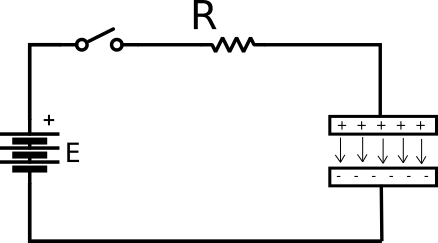
\includegraphics[scale=1]{images/capacitor_circuito_carga}
  \caption{Circuito de carga básico de un capacitor}
  \label{fig:cap_carga}
\end{figure}

Dado el circuito de la figura \ref{fig:cap_carga}, al cerrar el interruptor y por ahora omitiendo la resistencia (o suponiendo que posee una resistencia de $0 \Omega$), la placa inferior se comenzará a cargar con electrones libres, y la placa superior con cargas positivas.

Entre las placas, se alcanzará la tensión de la fuente $E$.

Como la distancia entre ambas es muy pequeña, las cargas se verán atraídas por una fuerza eléctrica (que recordando la ecuación \ref{eq:fuerza_electrica_capacitor}, será mayor si la distancia entre ambas es menor), y permanecerán atraídas incluso si se elimina la fuente de alimentación (o si se abre el circuito con el interruptor).

\begin{figure}[htbp]
  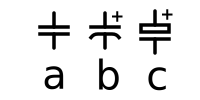
\includegraphics[scale=1]{images/capacitor_simbolo}
  \caption{Símbolos del capacitor: (a) No polarizado, (b) y (c) Polarizado}
  \label{fig:cap_simbolos}
\end{figure}

\subsubsection{Capacitancia}

La \textbf{capacitancia} de un capacitor es la cantidad de cargas que puede almacenar en él, cuando está completamente cargado.

\begin{equation}
	\label{eq:capacitancia}
	C = \frac{Q}{V}
\end{equation}

La unidad utilizada para medir la capacidad es el \textbf{Farad}, y 1 Farad de carga equivale a una carga de 1 Coulomb a una diferencia de potencial de 1 volt.
$$ 1 \text{Farad} = \frac{1 C}{1 V}$$

Redefiniendo la ecuación \ref{eq:fuerza_electrica_capacitor} para el caso del capacitor, resulta
\begin{equation}
	F_{ce} = \frac{V}{d}
\end{equation}

considerando la fuerza eléctrica en $Voltios/metro$, la tensión en $voltios$ y la distancia en $metros$.

El campo eléctrico también es afectado por la \textbf{permitividad} del material que se utiliza como dieléctrico. Un aumento en la permitividad del material, permitirá que la misma carga se almacene con un campo eléctrico menor; es decir, con un potencial eléctrico menor. Analizando la ecuación \ref{eq:capacitancia}, si la tensión disminuye, la capacitancia aumentará. En otras palabras, \textit{si la permitividad del dieléctrico es mayor, la capacidad será mayor}.

La permitividad $\epsilon $ se define como $ \epsilon = \frac{\epsilon_r}{\epsilon_0}$, donde $\epsilon_r$ es la permitividad relativa del material y $\epsilon_0 $ es la permitividad del vacío.

En la siguiente tabla, se recopilan los valores de algunos materiales utilizados para la construcción de dieléctricos de capacitores.

\begin{tabular}{|c|c|}
\hline 
Material & Permitividad relativa \\ 
\hline 
Aire & 1,0006 \\ 
\hline 
Papel & 1,5 \\ 
\hline 
Aceite & 2,8 \\ 
\hline 
Mica & 4 \\ 
\hline 
Cuarzo & 4,5 \\ 
\hline 
Baquelita & 5 \\ 
\hline 
PVC & 30 a 40 \\ 
\hline 
Agua destilada & 80 \\ 
\hline 
Acetona & 191 \\ 
\hline 
\end{tabular} 

Si se desea calcular la capacitancia teniendo en cuenta los valores de permitividad eléctrica, la ecuación es la siguiente,

\begin{equation}
	\label{eq:capacitancia_permitividad}
	C = \epsilon \frac{A}{d}
\end{equation}

considerando $\epsilon $ en $Farad/metro$, el área en metros cuadrados, la distancia en metros y la capacidad en Farads.

Debe tenerse en cuenta que los capacitores poseen un \textbf{voltaje de trabajo máximo}, que representa la máxima tensión que puede aplicarse en forma continua sin dañar el dispositivo. Si se excede, se puede dañar el dieléctrico.

\section{Campos magnéticos}
imán permanente, líneas de flujo magnético
densidad de flujo magnético
\subsection{Inductores}
\subsubsection{Construcción}
\subsubsection{Inductancia}
\subsubsection{Tensión inducida}
\subsubsection{Tipos de inductores}

\chapter{Corriente alterna}

Cuando en una gráfica de \textbf{tensión en función del tiempo} se observa un nivel de tensión por arriba del eje de abscisas, se considera positivo. Cuando está por debajo del eje, se considera negativo, y por lo tanto, representa a una corriente que está circulando en sentido contrario.
 
De esa manera, una tensión que se encuentre sin cruzar el eje en un determinado período de tiempo, se denomina \textbf{continua}. Si el sentido de la corriente cambia de forma periódica (es decir, pasa de negativa a positiva o viceversa, y se repite su forma de onda al transcurrir un determinado tiempo), se denomina \textbf{alterna}.
\begin{ejemplo}
	En las imágenes se pueden apreciar distintas variaciones de la tensión a lo largo del tiempo.
	\begin{itemize}
		\item En la \textbf{figura \ref{fig:acdc_a}}, la tensión es continua.
		\item En la \textbf{figura \ref{fig:acdc_b}}, la tensión es alterna, y tiene una forma de onda cuadrada.
		\item En la \textbf{figura \ref{fig:acdc_c}}, la tensión es alterna, y tiene una forma de onda senoidal.
		\item En la \textbf{figura \ref{fig:acdc_d}}, la tensión, si bien tiene forma de onda senoidal, es continua, porque se encuentra siempre por arriba del eje de abscisas. En otras palabras: nunca cambia su sentido, sino que sólo varía su valor de tensión.
	\end{itemize}
\end{ejemplo}

\begin{figure}[htbp]
  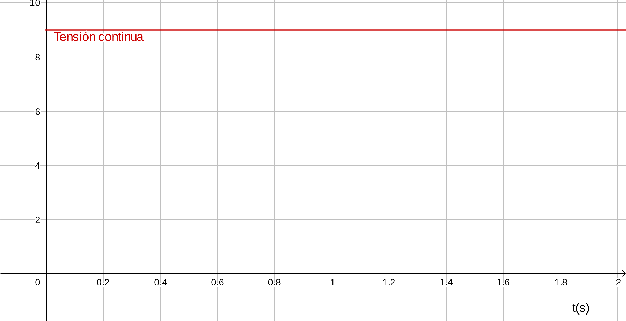
\includegraphics[scale=0.75]{images/acdc_a}
  \caption{Corriente continua}
  \label{fig:acdc_a}
\end{figure}
\begin{figure}[htbp]
  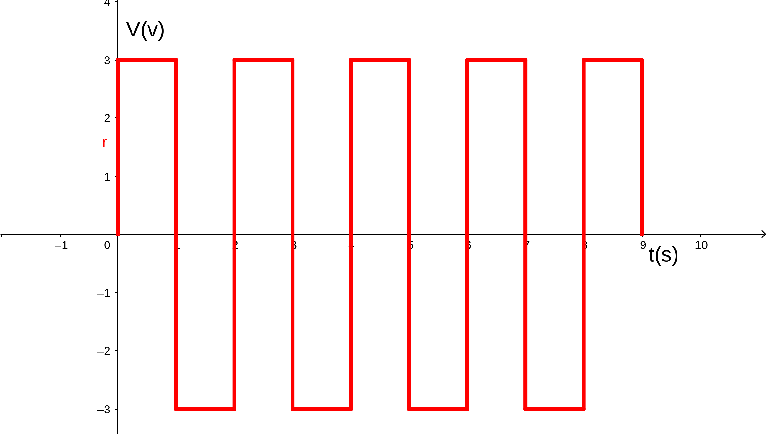
\includegraphics[scale=0.6]{images/acdc_b}
  \caption{Corriente alterna cuadrada}
  \label{fig:acdc_b}
\end{figure}
\begin{figure}[htbp]
  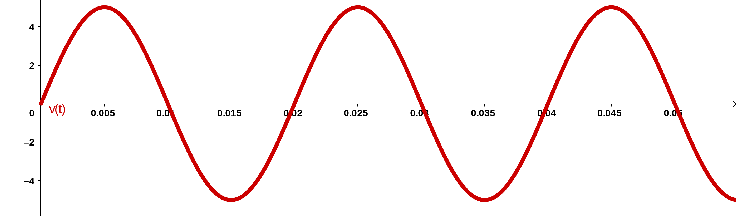
\includegraphics[scale=0.14]{images/acdc_c}
  \caption{Corriente alterna senoidal}
  \label{fig:acdc_c}
\end{figure}
\begin{figure}[htbp]
  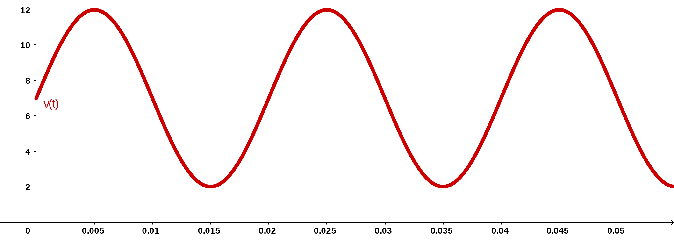
\includegraphics[scale=0.6]{images/acdc_d}
  \caption{Corriente con forma senoidal no alterna}
  \label{fig:acdc_d}
\end{figure}
Si bien existen varias formas de ondas de corriente alterna (triangular, cuadrada), la más difundida es la \textbf{forma senoidal}, que se puede apreciar en la figura \ref{fig:acdc_c}. Esto es así, porque es el voltaje que se genera en las plantas eléctricas y porque, además, permite realizar ciertos cálculos matemáticos que la explican y predicen, aunque son algo más complejos que los de corriente directa o continua.

\section{Corriente alterna senoidal}

En la figura \ref{fig:ac} se puede distinguir una onda alterna senoidal. Pueden distinguirse los siguientes parámetros:

\begin{itemize}
	\item Valor instantáneo: magnitud de una forma de onda en cualquier instante. Se han indicado como ejemplos $e_1$, $e_2$ y $e_3$.
	\item Valor pico: valor instantáneo máximo medido con respecto al nivel de 0 Volts. En la gráfica, se indicó como $Vp$. También se indicó el valor de pico negativo como $-Vp$.
	\item Valor pico a pico: tensión entre $Vp$ y $-Vp$. Es la suma entre las magnitudes de los valores de pico positivo y negativo.
	\item Ciclo: parte más pequeña de una onda hasta que comienza a repetirse.	
	\item Periodo $T$: Tiempo que dura un ciclo. En el ejemplo se tiene 3 periodos (de $O$ a $T_1$, de $T_1$ a $T_2$ y de $T_2$ a $T_3$, aunque pueden indicarse otros periodos).
	\item Frecuencia $f$: es la cantidad de ciclos que ocurren en 1 segundo. La frecuencia se mide en hertz (Hz), donde $1\; Hertz = 1\; \text{ciclo por segundo}$.
\end{itemize}

Del desarrollo anterior, se desprende que:
\begin{equation}
	\label{eq:frec_ciclos}
	f=\frac{1}{T}
\end{equation}
Y que:
\begin{equation}
	\label{eq:ciclos_frec}
	T=\frac{1}{f}
\end{equation}
Donde \textbf{T} se mide en segundos, y \textbf{$f$} se mide en Hz (Hertz).
\begin{figure}[htbp]
  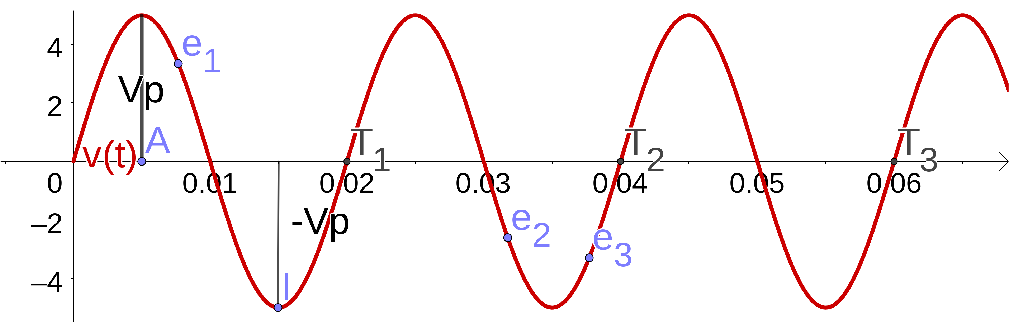
\includegraphics[scale=0.14]{images/ac}
  \caption{Corriente alterna senoidal: parámetros}
  \label{fig:ac}
\end{figure}
\begin{ejemplo}
	\label{ej:ac_argentina}
	En la figura \ref{fig:ac_argentina} se puede apreciar una onda senoidal que representa la tensión utilizada en Argentina.
	
	El valor de pico es $Vp = 311\; V$ y el periodo $T = 0,02\; s$.
	
	La frecuencia es $$f=\frac{1}{0,02\; s}=50\; Hz$$
	
	El valor de pico a pico es $$ Vpp = 2 \times 311\; V = 622\; V $$
\end{ejemplo}
\begin{figure}[htbp]
  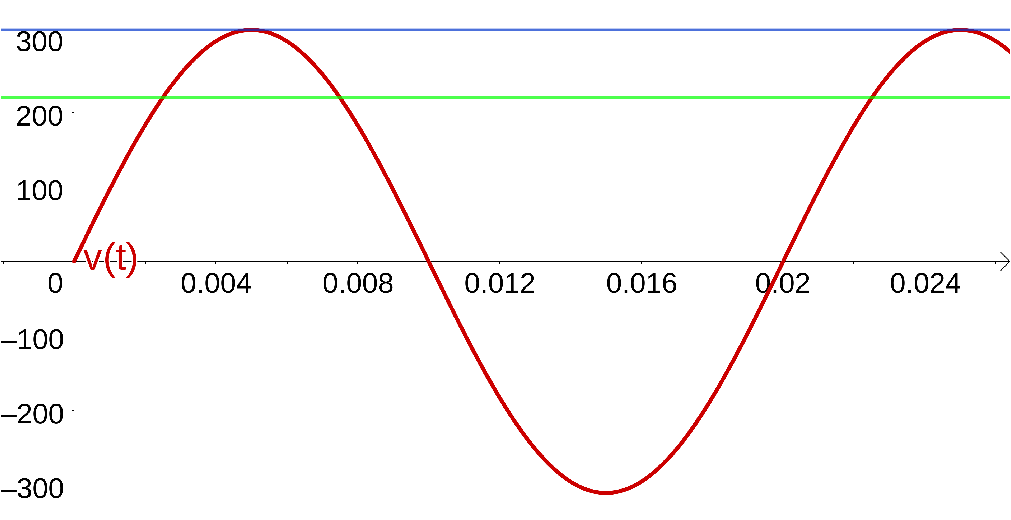
\includegraphics[scale=0.1]{images/ac_argentina}
  \caption{Corriente alterna en Argentina. En color azul, la tensión de pico y en color verde, la tensión eficaz}
  \label{fig:ac_argentina}
\end{figure}

\subsection{Definición matemática}
Si se desea considerar a la tensión (en voltios) en función del tiempo (en segundos) para una forma de onda senoidal, se deberá partir de la función $$v(\alpha) = sen (\alpha) $$
Obsérvese que en vez de utilizarse la variable $t$ (que se suele utilizar para indicar tiempo como número real), se ha definido un ángulo $\alpha$. Esto se debe a que la función senoidal está definida como el conjunto de valores que se obtienen al proyectar verticalmente un vector de radio que gira con movimiento circular uniforme alrededor de un punto fijo. La forma senoidal completa se trazará luego de haber completado una rotación de 360 grados alrededor del centro (o $2\pi$ radianes).

Suele ser más cómodo trabajar con \textbf{radianes} en vez de \textbf{grados sexagesimales} para medir los ángulos y es lo que se hará en este texto.

La idea de \textbf{proyectar verticalmente} el vector proviene de la trigonometría, ya que el $sen \alpha = \frac{\text{cateto opuesto}}{\text{radio}}$, como puede apreciarse en la figura \ref{fig:seno_triangulo}. Como el radio del vector es 1, entonces $ sen \alpha = \text{cateto opuesto} $, que es la \textbf{proyección vertical} del vector.

\begin{figure}[htbp]
  \includegraphics[scale=0.1]{images/seno_triangulo}
  \caption{Seno en un triángulo rectángulo}
  \label{fig:seno_triangulo}
\end{figure}

Un desarrollo de esta idea puede apreciarse en la figura \ref{fig:seno_proyectado}.
\begin{figure}[htbp]
%  \includegraphics[scale=1]{}
  \caption{Forma de onda senoidal a partir de la proyección de un radio versor}
  \label{fig:seno_proyectado}
\end{figure}

El vector gira con una velocidad angular $\omega$ alrededor del centro, determinada por la ecuación $$\omega = \frac{\text{distancia}}{\text{tiempo}}= \frac{\alpha}{t}$$ lo cual implica que $$ \omega t = \alpha $$

Como una vuelta completa se realiza en un periodo $T$ (que a su vez tarda 360 grados o $2 \pi$ en realizarse), se puede decir que 
$$\omega = \frac{2\pi}{T}$$ o bien, si se utiliza la ecuación \ref{eq:frec_ciclos}, $$\omega = 2\pi f$$

Volviendo a la ecuación de la tensión en función del tiempo, podría redefinirse como $$v(t) = sen (\omega t)$$, permitiendo expresar, ahora sí, la tensión en función del tiempo.

Sólo falta un detalle... debe observarse que el valor de pico de esta onda es el mismo que el del radio vector (1). Por lo tanto, la forma final de la onda seno que representa a la tensión en función del tiempo, deberá estar multiplicada por el valor de pico, de la siguiente forma: 
\begin{equation}
	\label{eq:senoidal}
	v(t) = Vp \times sen(\omega t)
\end{equation}

\subsection{Relaciones de fase}
Si la onda se desplaza $\theta$ grados, la expresión de la tensión se vuelve 
$$v=Vp \times sen (\omega t \pm \theta ) $$

Si se comparan dos ondas senoidales de la \textbf{misma frecuencia}, pueden indicarse relaciones de \textbf{adelanto} o de \textbf{atraso} de una con respecto a la otra.

\begin{ejemplo}
	En la figura \ref{fig:ejemplos_senos} puede apreciarse la función $v(t)=sen(\omega t)$ en color rojo y en color azul la función $v(t)=cos(\omega t)$. Nótese que la forma de onda es exactamente igual al seno, pero con un desplazamiento en el eje horizontal: esto es lo que habitualmente se denomina \textbf{desfasaje}. De ese modo, el coseno se podría redefinir como un seno desplazado, o viceversa: $$ sen(\alpha) = cos(\alpha - 90º) $$ $$ cos(\alpha) = sen(\alpha + 90º) $$
	Puede apreciarse en la figura, la función $sen(\omega t -90º)$ en color verde. Nótese que si el ángulo de desplazamiento es positivo, como en el ejemplo anterior, la curva se desplaza hacia la izquierda, y si el ángulo es negativo, como en este caso, el desplazamiento es hacia la derecha.
\end{ejemplo}

\begin{figure}[htbp]
  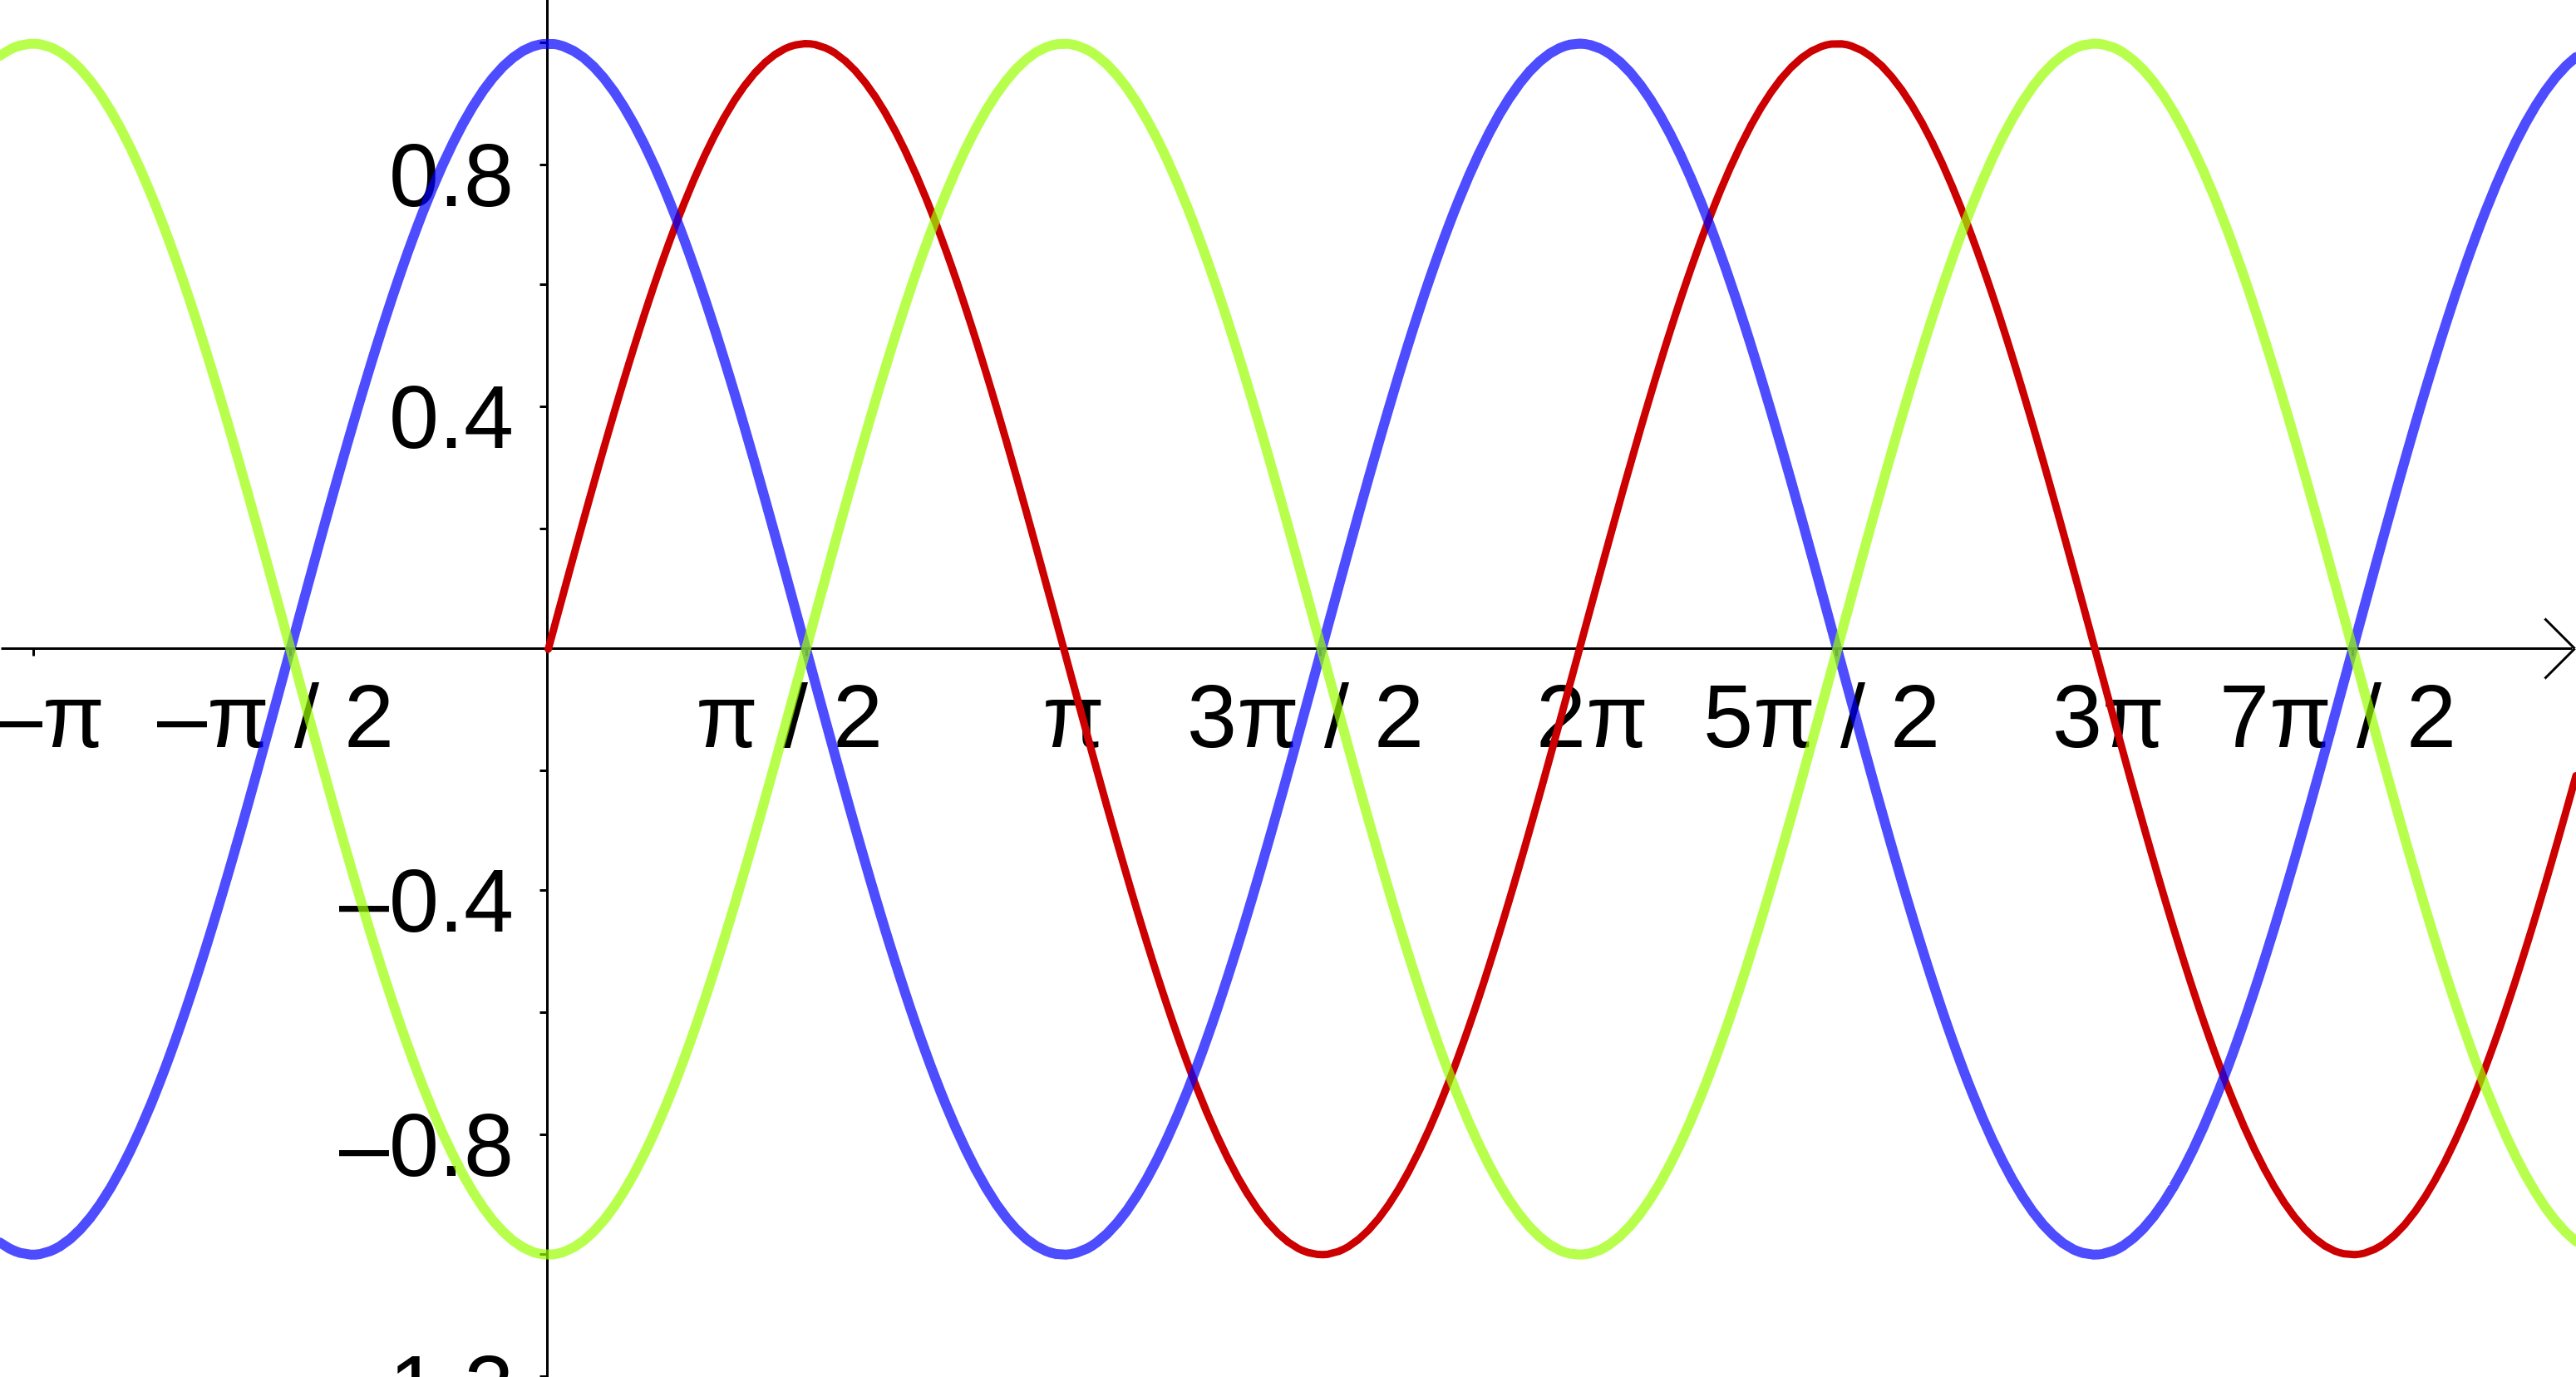
\includegraphics[scale=0.14]{images/ejemplos_senos}
  \caption{Ondas desfasadas}
  \label{fig:ejemplos_senos}
\end{figure}

\section{Valores rms}
El \textbf{valor RMS} o \textbf{valor eficaz}, es el valor de tensión o corriente alterna que produce la misma potencia que su equivalente en corriente continua.

No debe confundirse el valor eficaz con el \textbf{valor promedio}. El valor promedio de una tensión es la suma algebraica de las áreas respecto de la longitud de la curva. Si se analiza la corriente alterna senoidal, se observará que el valor promedio de tensión es de $0\; V$. No ocurre lo mismo con la \textbf{tensión eficaz}.

\begin{figure}[htbp]
  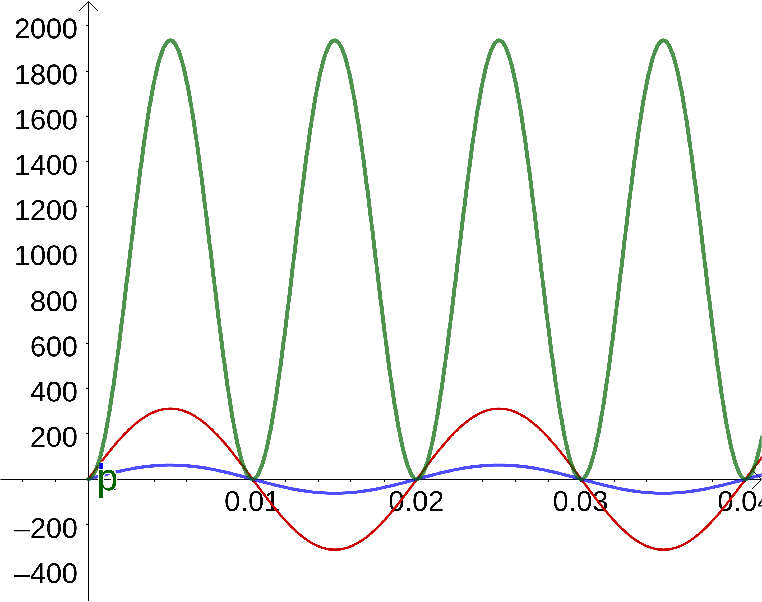
\includegraphics[scale=0.14]{images/potencia_alterna}
  \caption{Entrega de potencia en una corriente alterna senoidal}
  \label{fig:potencia_alterna}
\end{figure}

Al analizar la figura \ref{fig:potencia_alterna}, se puede observar tres ondas senoidales en fase. La más pequeña (azul), corresponde a la corriente eléctrica, medida en Amperes. La onda intermedia es la tensión (roja), expresada en Voltios. Estas ondas, poseen un semiciclo positivo y un semiciclo negativo, lo que indica un cambio en el sentido de la corriente.

La onda que toma mayor amplitud (verde), es la \textbf{potencia entregada}, calculada como el producto entre la tensión y la corriente eléctrica. Como se puede observar, todo el tiempo es positiva (excepto en los instantes 0, 0,1s y 0,2s).

Entonces, el problema de hallar la tensión eficaz, reside en observar para qué valor de tensión continua, la potencia entregada sería la misma que la de la onda más grande (verde) de la figura \ref{fig:potencia_alterna}.

A continuación se supondrá que se aplica una tensión con valor de pico $Vp$ y corriente de pico $Ip$ sobre una resistencia $R$.

\begin{eqnarray*}
	p(t)= i(t)^{2} R \\
	p(t)= [Ip sen(\omega t)]^{2} R \\
	p(t)= Ip^{2}sen^{2}(\omega t)R \\
\end{eqnarray*}
En este punto se utiliza la identidad trigonométrica $sen^{2}(\omega t) = \frac{1}{2}(1-cos(2\omega t))$.
\begin{eqnarray*}
	p(t)= Ip^{2}[\frac{1}{2}(1-cos(2 \omega t))]R \\
	p(t)=\frac{Ip^{2}R}{2}-\frac{Ip^{2}R}{2}cos(2 \omega t)
\end{eqnarray*}
Se anula el segundo término  por poseer valor medio igual a 0
 $$	p(t)=\frac{Ip^{2}R}{2} $$

Como se desea evaluar el valor de corriente continua equivalente, se supondrá que ahora se aplicó una corriente directa $I_{DC}$ a la misma carga resistiva. Su potencia $P_{DC}$ se calcularía de la siguiente forma:

$$ P_{DC} = I_{DC}^{2}R $$

Al igualar $P_{DC}$ con $p(t)$, se obtiene:
\begin{eqnarray*}
	p(t)=P_{DC} \\
	\frac{Ip^{2}R}{2}=I_{DC}^{2}R \\
	I_{DC}=\frac{Ip}{\sqrt{2}}=0,707Ip
\end{eqnarray*}

Es decir, que el valor de corriente continua equivalente de una corriente senoidal alterna es 0,707 su valor de pico. Este mismo análisis puede realizarse con la tensión, obteniendo el mismo valor.

Mediante el cálculo se puede demostrar a través de la integración, pero excede los temas de este curso.

\begin{conclusiones}
	Las siguientes ecuaciones permiten hallar valores eficaces a partir de valores de pico.
	\begin{equation}
		I_{RMS} = \frac{1}{\sqrt{2}}I_{PICO}=I_{PICO}\times 0,707
	\end{equation}
	\begin{equation}
		V_{RMS} = \frac{1}{\sqrt{2}}V_{PICO}=V_{PICO}\times 0,707
	\end{equation}
	Las siguientes ecuaciones, despejadas de las anteriores, permiten encontrar valores de pico a partir de valores eficaces.
	\begin{equation}
		I_{PICO} = \sqrt{2}I_{RMS}=I_{RMS}\times 1,414
	\end{equation}
	\begin{equation}
		V_{PICO} = \sqrt{2}V_{RMS}=V_{RMS}\times 1,414
	\end{equation}
\end{conclusiones}

\section{Respuesta en frecuencia}

Una vez ha transcurrido el periodo transitorio en capacitores e inductores, puede analizarse estos componentes como se describe en esta sección.

\subsection{Respuesta del resistor}

Para frecuencias de línea ($50\; Hz$ en el caso de Argentina), las cargas resistivas tienen un comportamiento lineal, y por ello puede aplicarse directamente la Ley de Ohm para calcular sus tensiones y corrientes.

\begin{figure}[htbp]
%  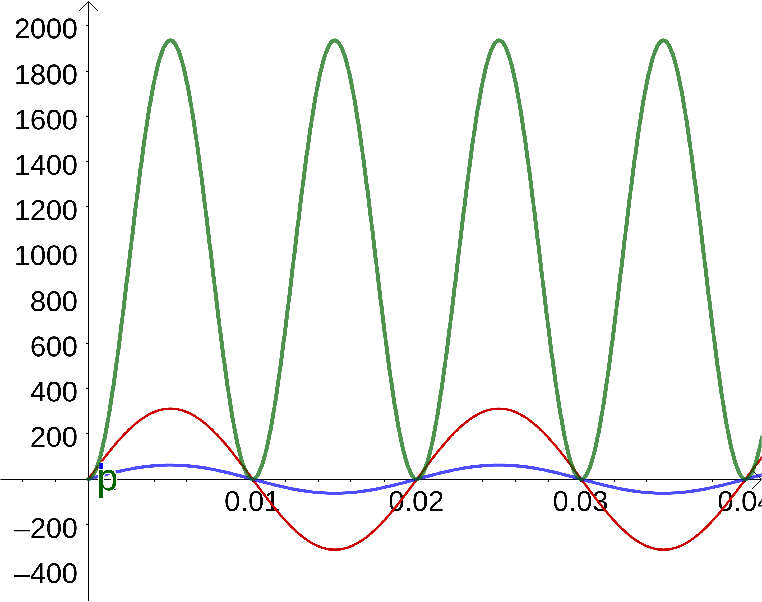
\includegraphics[scale=0.14]{images/potencia_alterna}
  \caption{Curvas de respuesta del resistor en corriente alterna}
  \label{fig:respuesta_resistor_curvas}
\end{figure}
\begin{figure}[htbp]
%  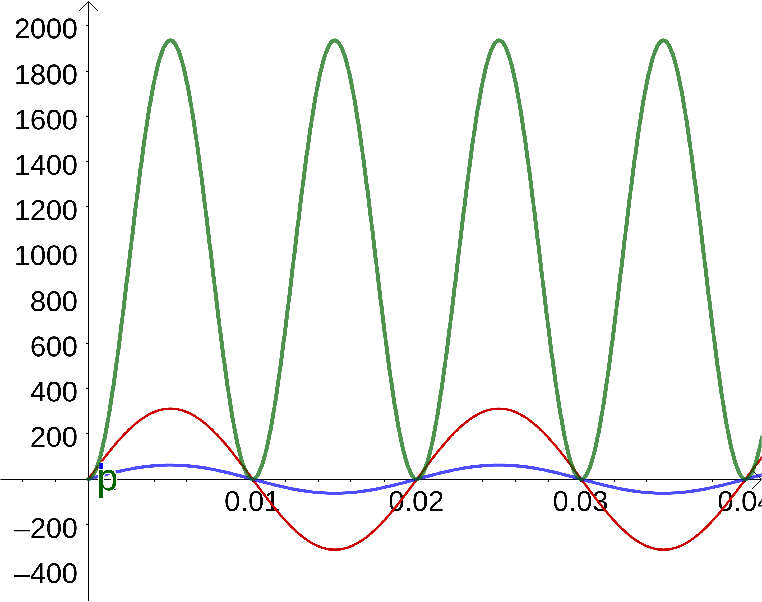
\includegraphics[scale=0.14]{images/potencia_alterna}
  \caption{Circuito resistivo con una fuente de corriente alterna}
  \label{fig:respuesta_resistor_circuito}
\end{figure}

$$ i = \frac{V_{RMS} \times sen(\omega t)}{R} = \frac{V_{RMS}}{R} sen(\omega t) = I_{RMS} sen(\omega t) $$

Como se observa en la figura~\ref{fig:respuesta_resistor_curvas}, la fase de la corriente y la tensión es la misma. Por lo tanto, la variación de corriente y tensión ocurren en la misma proporción y puede considerarse:

\begin{equation}
	\label{eq:i_resistor_alterna}
	I_{RMS} = \frac{V_{RMS}}{R}
\end{equation}
\begin{equation}
	\label{eq:i_resistor_alterna}
	V_{RMS} = I_{RMS}\times R
\end{equation}

\subsection{Respuesta del inductor}

La tensión a través de un inductor está directamente relacionado con la velocidad de cambio de la corriente a través del mismo. En corriente alterna, esta variación está dada, entre otros factores, por la frecuencia de la red. Por ello, existe una relación entre la frecuencia, la tensión en el inductor y su valor de inductancia.

\begin{eqnarray*}
	v_L = L \frac{di_L}{dt} \\
	v_L = L \frac{d}{dt}(Ip\times sen(\omega t)) \\
	v_L = L( \omega Ip\times cos (\omega t)) \\
	v_L = \omega L Ip\times cos(\omega t) \\
	v_L = \omega L Ip\times sen(\omega t +90^{\circ}) \\
\end{eqnarray*}

Como se explicó antes, el valor de pico está relacionado con $\omega=2\pi f$, y por $L$ como se explicó anteriormente. También puede apreciarse que la corriente y la tensión difieren en su fase por 90º.

\begin{conclusiones}
	En el inductor, la tensión $v_L$ va por delante 90º a la corriente $i_L$. 
	\begin{equation}
		\label{eq:i_inductor}
		i_L = Ip\times sen(\omega t)
	\end{equation}
	
	\begin{equation}
		\label{eq:v_inductor}
		v_L = \omega \times L \times Ip \times sen(\omega t + 90^{\circ})
	\end{equation}
	
\end{conclusiones}

\subsection{Respuesta del capacitor}

La tensión en un capacitor está limitada por la velocidad a la cual se depositan o liberan las cargas entre sus placas, y por ello, a mayor frecuencia, mayor corriente.

Por otra parte, mientras mayor sea el valor de capacitancia, mayor será la corriente capacitiva resultante, debido a que $i = C(dv/dt)$.

\begin{eqnarray*}
	i_C = C \frac{dv_C}{dt} \\
	i_C = C \frac{d}{dt}(Vp\times sen(\omega t)) \\
	i_C = C (\omega \times Vp \times cos(\omega t)) \\
	i_C = \omega \times C \times Vp \times sen(\omega t + 90^{\circ}) \\
\end{eqnarray*}

\begin{conclusiones}
	En el capacitor, la corriente $i_C$ va por delante a la tensión $v_C$ unos 90º. 
	\begin{equation}
		\label{eq:v_capacitor}
		v_C = Vp\times sen(\omega t)
	\end{equation}
	\begin{equation}
		\label{eq:i_capacitor}
		i_C = \omega \times C \times Vp \times sen(\omega t + 90^{\circ})
	\end{equation}
\end{conclusiones}



\subsection{Impedancia}

La \textbf{oposición} en un circuito de corriente alterna, está dada por la Ley de Ohm. Ocurre que, al incorporar capacitancias e inductancias, la idea de \textbf{resistencia} resulta insuficiente para modelar la oposición.

Si se vuelve a analizar lo expuesto en este capítulo según la relación $\text{Efecto} = \frac{\text{Causa}}{\text{Oposición}} \rightarrow \text{Oposición} = \frac{\text{Causa}}{\text{Efecto}}$, como se ha hecho anteriormente, y volviendo a suponer a la corriente como el \textbf{efecto} que produce la \textbf{tensión}, se puede abordar la idea de \textbf{impedancia}, definida como \textit{la oposición que presenta un circuito de de corriente alterna al aplicarle una tensión}.

\begin{equation}
	\label{eq:impedancia}
	Z=\frac{V}{I}
\end{equation}

En la ecuación \ref{eq:impedancia}, $Z$ refiere a la impedancia, y tanto $V$ como $I$ son fasores (números complejos que representan a la tensión y corriente alterna respectivamente).

La impedancia, cuyo término proviene de la idea de \textit{impedir el paso de la corriente}, estará compuesta por una parte \textbf{resistiva}, y una parte \textbf{reactiva} (que \textit{reacciona}, o no sólo consume energía sino que también puede almacenarla y devolverla eventualmente). Los componentes \textbf{reactivos} serán los inductores y los capacitores.

Para el caso del inductor, según las ecuaciones \ref{eq:i_inductor} y \ref{eq:v_inductor}, se define a la oposición del mismo como \textbf{reactancia inductiva $X_L$} de la siguiente forma:

$$ X_L = \frac{\omega \times L \times Ip \times sen(\omega t)}{Ip\times sen(\omega t)} = \omega L $$

De manera análoga, para el capacitor y según las ecuaciones \ref{eq:i_capacitor} y \ref{eq:v_capacitor}, se define como \textbf{reactancia capacitiva $X_C$} a:

$$ X_C = \frac{Vp\times sen(\omega t)}{\omega \times C \times Vp \times sen(\omega t)} = \frac{1}{\omega C} $$

La \textbf{impedancia Z}, puede ser definida como un fasor que relaciona la \textbf{resistencia} con la \textbf{reactancia} de la siguiente forma:

\begin{equation}
	\label{eq:impedancia_rectangular}
	Z = R + j(X_L-X_C)
\end{equation}

\section{Fasores}
Los fasores permiten relacionar tensiones y corrientes alternas senoidales de una forma más sencilla que si se trabajara directamente con las ondas.

Como ya se sabe, una onda senoidal se define completamente por su \textbf{amplitud}, \textbf{frecuencia} y \textbf{fase}. Como se trabajará siempre con la misma frecuencia, sólo se necesitará la amplitud y la fase para poder definirlas, y ésto se puede hacer a través de vectores, que se llamarán fasores.

%Un \textbf{fasor} es un número complejo que tiene como variable a su argumento.
%$$ U = | U | e^{j\omega t} $$
%Aplicando la fórmula de Euler en la expresión anterior, resulta,
%$$ U = | U | cos (\omega t) + j|U| sen(\omega t) $$

Un \textbf{fasor} es un vector giratorio que permite representar una onda de corriente o de tensión. El módulo del vector representa el valor eficaz de la onda, mientras que la frecuencia será la velocidad a la que giran (cuestión que será omitida, porque se supone que todos giran a la misma velocidad angular), y la fase está representada por el ángulo entre fasores.

En otras palabras, los fasores representan una fotografía instantánea de la posición del vector giratorio que define las ondas de tensión y de corriente.

La impedancia, también es un número complejo y fasor, definido como $Z= R+j(X_L - X_C)$, y $X_L = \omega L $, $X_C = \frac{1}{\omega C}$, como se ha visto anteriormente. La diferencia con los fasores de tensión y de corriente, es que la impedancia no se encuentra girando sino que está estática.

Para realizar operaciones con fasores (lo cual es más sencillo que operar con ecuaciones de ondas), se debe utilizar el álgebra de los números complejos, resultando más conveniente utilizar la \textbf{forma rectangular} para realizar sumas y restas, y la \textbf{forma polar} para realizar multiplicaciones y divisiones.

\subsection{Síntesis de álgebra de complejos}

Un estudio completo de números complejos excede el contenido de este apunte. Se limitará a sintetizar las técnicas necesarias para trabajar con fasores.

\subsubsection{Conversión rectangular a polar}

Dado un vector $v$ con módulo $|V|$ y ángulo $\theta$, con $a$ como su componente en $x$ y $b$ como su componente en $y$, puede representarse dicho vector como el número complejo $a+jb$, donde $j$ es la unidad imaginaria (no se utiliza $i$ para no confundirlo con la corriente eléctrica).



\section{Potencia}

La ecuación general de la potencia es: $$ p = vi $$

Nótese que las tres magnitudes varían en el tiempo (y por ello están escritas en minúscula). Para el caso de corriente continua, bastaría con operar utilizando la ecuación  \ref{eq:pot}, pero cuando se trata de una corriente alterna senoidal, este cálculo es algo más complejo, y más aún cuando existen desfasajes entre la tensión y la corriente aplicada a la carga.

En corriente alterna se definen tres tipos de potencia: la activa, reactiva y aparente, y a su vez, se introduce un factor de potencia.

La \textbf{potencia activa} es la que consume cualquier aparato eléctrico para funcionar, y se mide en Watts ($W$).

En corriente alterna las bobinas y los condensadores no sólo consumen energía, sino que también la acumulan. Entonces, una cierta cantidad de potencia se mueve dentro del circuito pero no sale de él, y recibe el nombre de \textbf{potencia reactiva}. Éste tipo de potencia se mide en Volt-Amperes reactivos ($VAr$).

En el caso de la potencia reactiva, no hay un real consumo de energía, ya que primero se consume y luego se devuelve, pero este fenómeno implica que el proveedor de energía deba entregar toda esta potencia (la activa y también la reactiva, aunque luego ésta última vaya a ser devuelta), con su consecuente necesidad de dimensionar los conductores para un consumo mayor. Pareciera ser que, como la potencia reactiva no es disipada, entonces no  debería ser tenida en cuenta, pero para el proveedor de energía es importante, ya que debe entregarla de todos modos, aunque luego sea devuelta. Desde el punto de vista del consumidor, una parte de la energía se pide ``prestada" para hacer funcionar elementos con consumos reactivos (como motores o transformadores) y luego se devuelve a la red, pero de todos modos, aunque esta energía no haya sido parte de la energía aprovechada por los elementos de la red, fue necesaria para hacerlos funcionar correctamente.

La \textbf{potencia aparente} corresponde a la energía que se entrega por el proveedor, que no sólo expresa el valor de potencia activa sino también a la potencia reactiva. Esto llevaría a pensar que la potencia aparente es simplemente la suma de ambas potencias, pero debe recordarse que en corriente alterna, ambos valores corresponden a ondas, y por lo tanto su cálculo no es tan simple de realizar. La unidad que se utiliza para medir la potencia aparente es el Volt-Ampere ($VA$).

A continuación, se muestran imágenes para distintos tipos de consumo.
\begin{itemize}
	\item Para el consumo resistivo puro de la figura \ref{fig:potencia_alterna_resistiva}, las ondas de corriente y de tensión están en fase. La potencia será el producto entre ambas, y como se observa en la gráfica, siempre es positiva (está por arriba del eje de abscisas). Esto significa que siempre se está entregando potencia activa.
	\item En los consumos capacitivo puro e inductivo puro de las figuras \ref{fig:potencia_alterna_capacitiva} y \ref{fig:potencia_alterna_inductiva} respectivamente, puede apreciarse que durante medio ciclo de potencia, el sistema entrega potencia, pero la otra mitad de tiempo la absorbe. En otras palabras, la potencia activa es de $0\; W$, porque nunca se está disipando energía, y la potencia es puramente reactiva.
	\item En las curvas de la figura \ref{fig:potencia_alterna_mixta}, se observa un consumo real, que es en parte reactivo y en parte activo, pero la parte activa es mayor que la reactiva. Es decir, que la potencia entregada es mayor a la potencia devuelta. Esto es lo que ocurre en las redes eléctricas reales.
\end{itemize}
% Imágenes de consumo resistivo, inductivo, capacitivo y mixto.
\begin{figure}[htbp]
  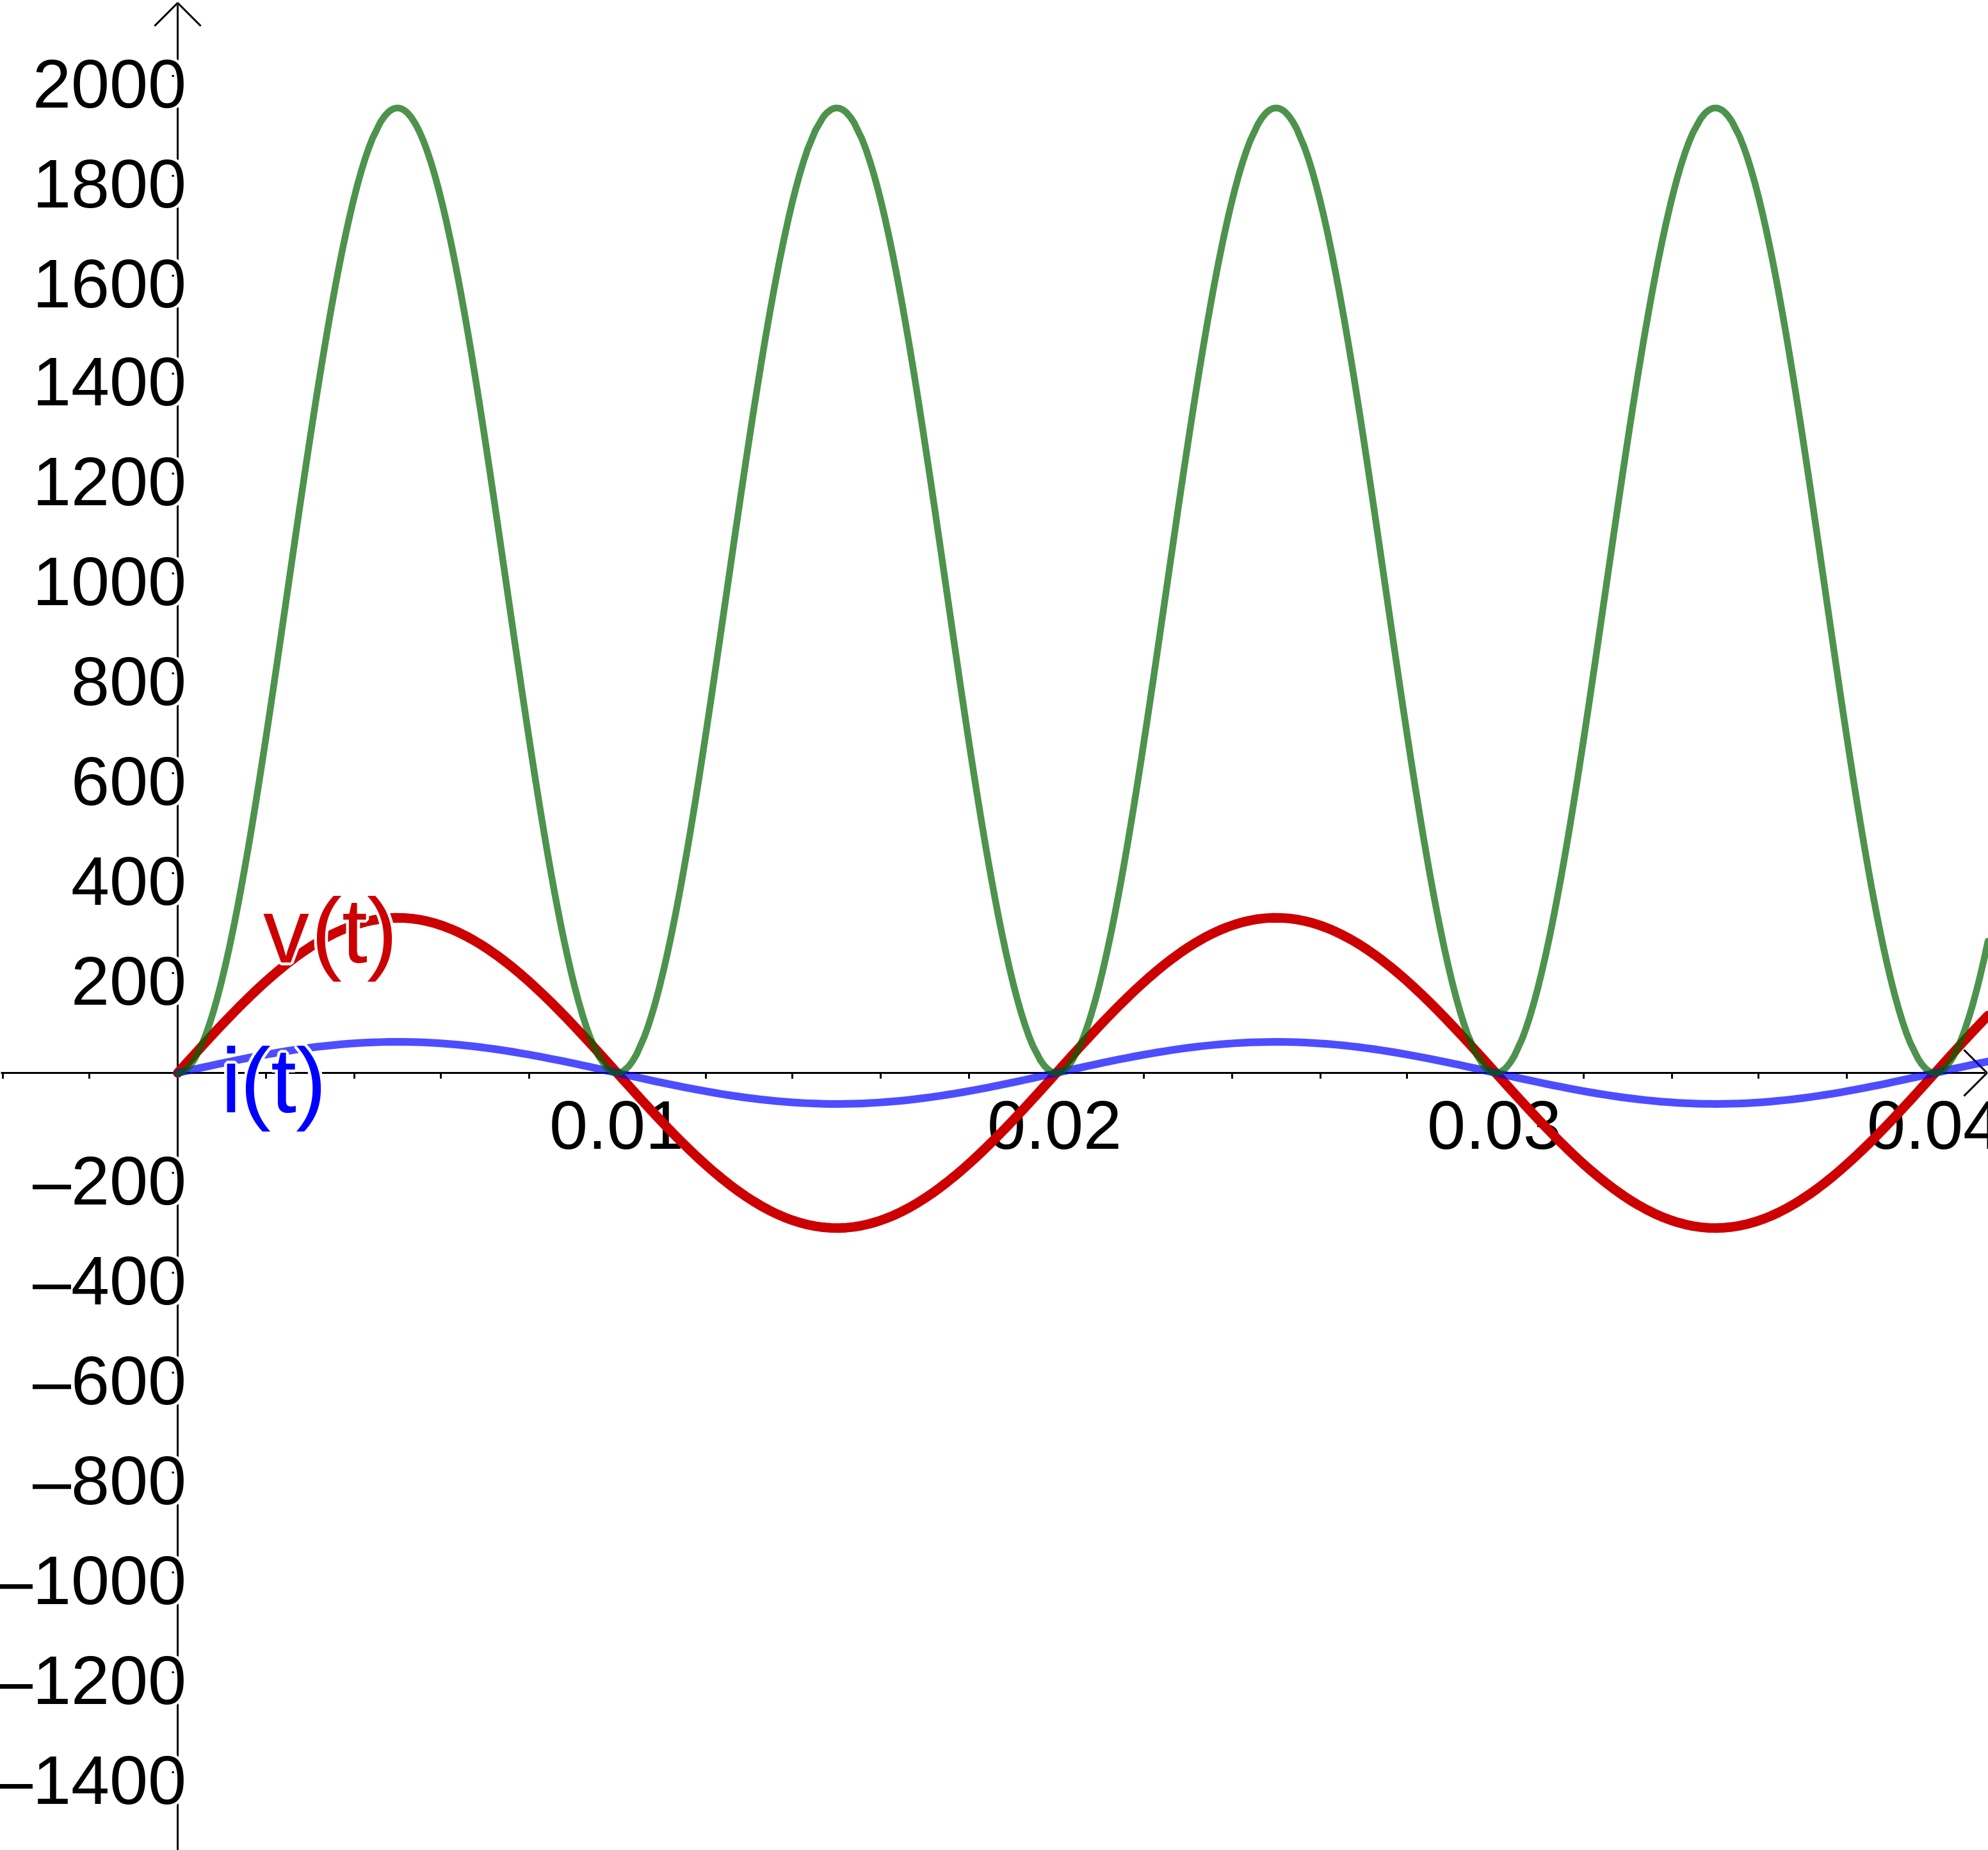
\includegraphics[scale=0.1]{images/potencia_alterna_resistiva}
  \caption{Respuesta de un circuito resistivo puro en C.A.: corriente en azul, tensión en rojo y potencia en verde}
  \label{fig:potencia_alterna_resistiva}
\end{figure}

\begin{figure}[htbp]
  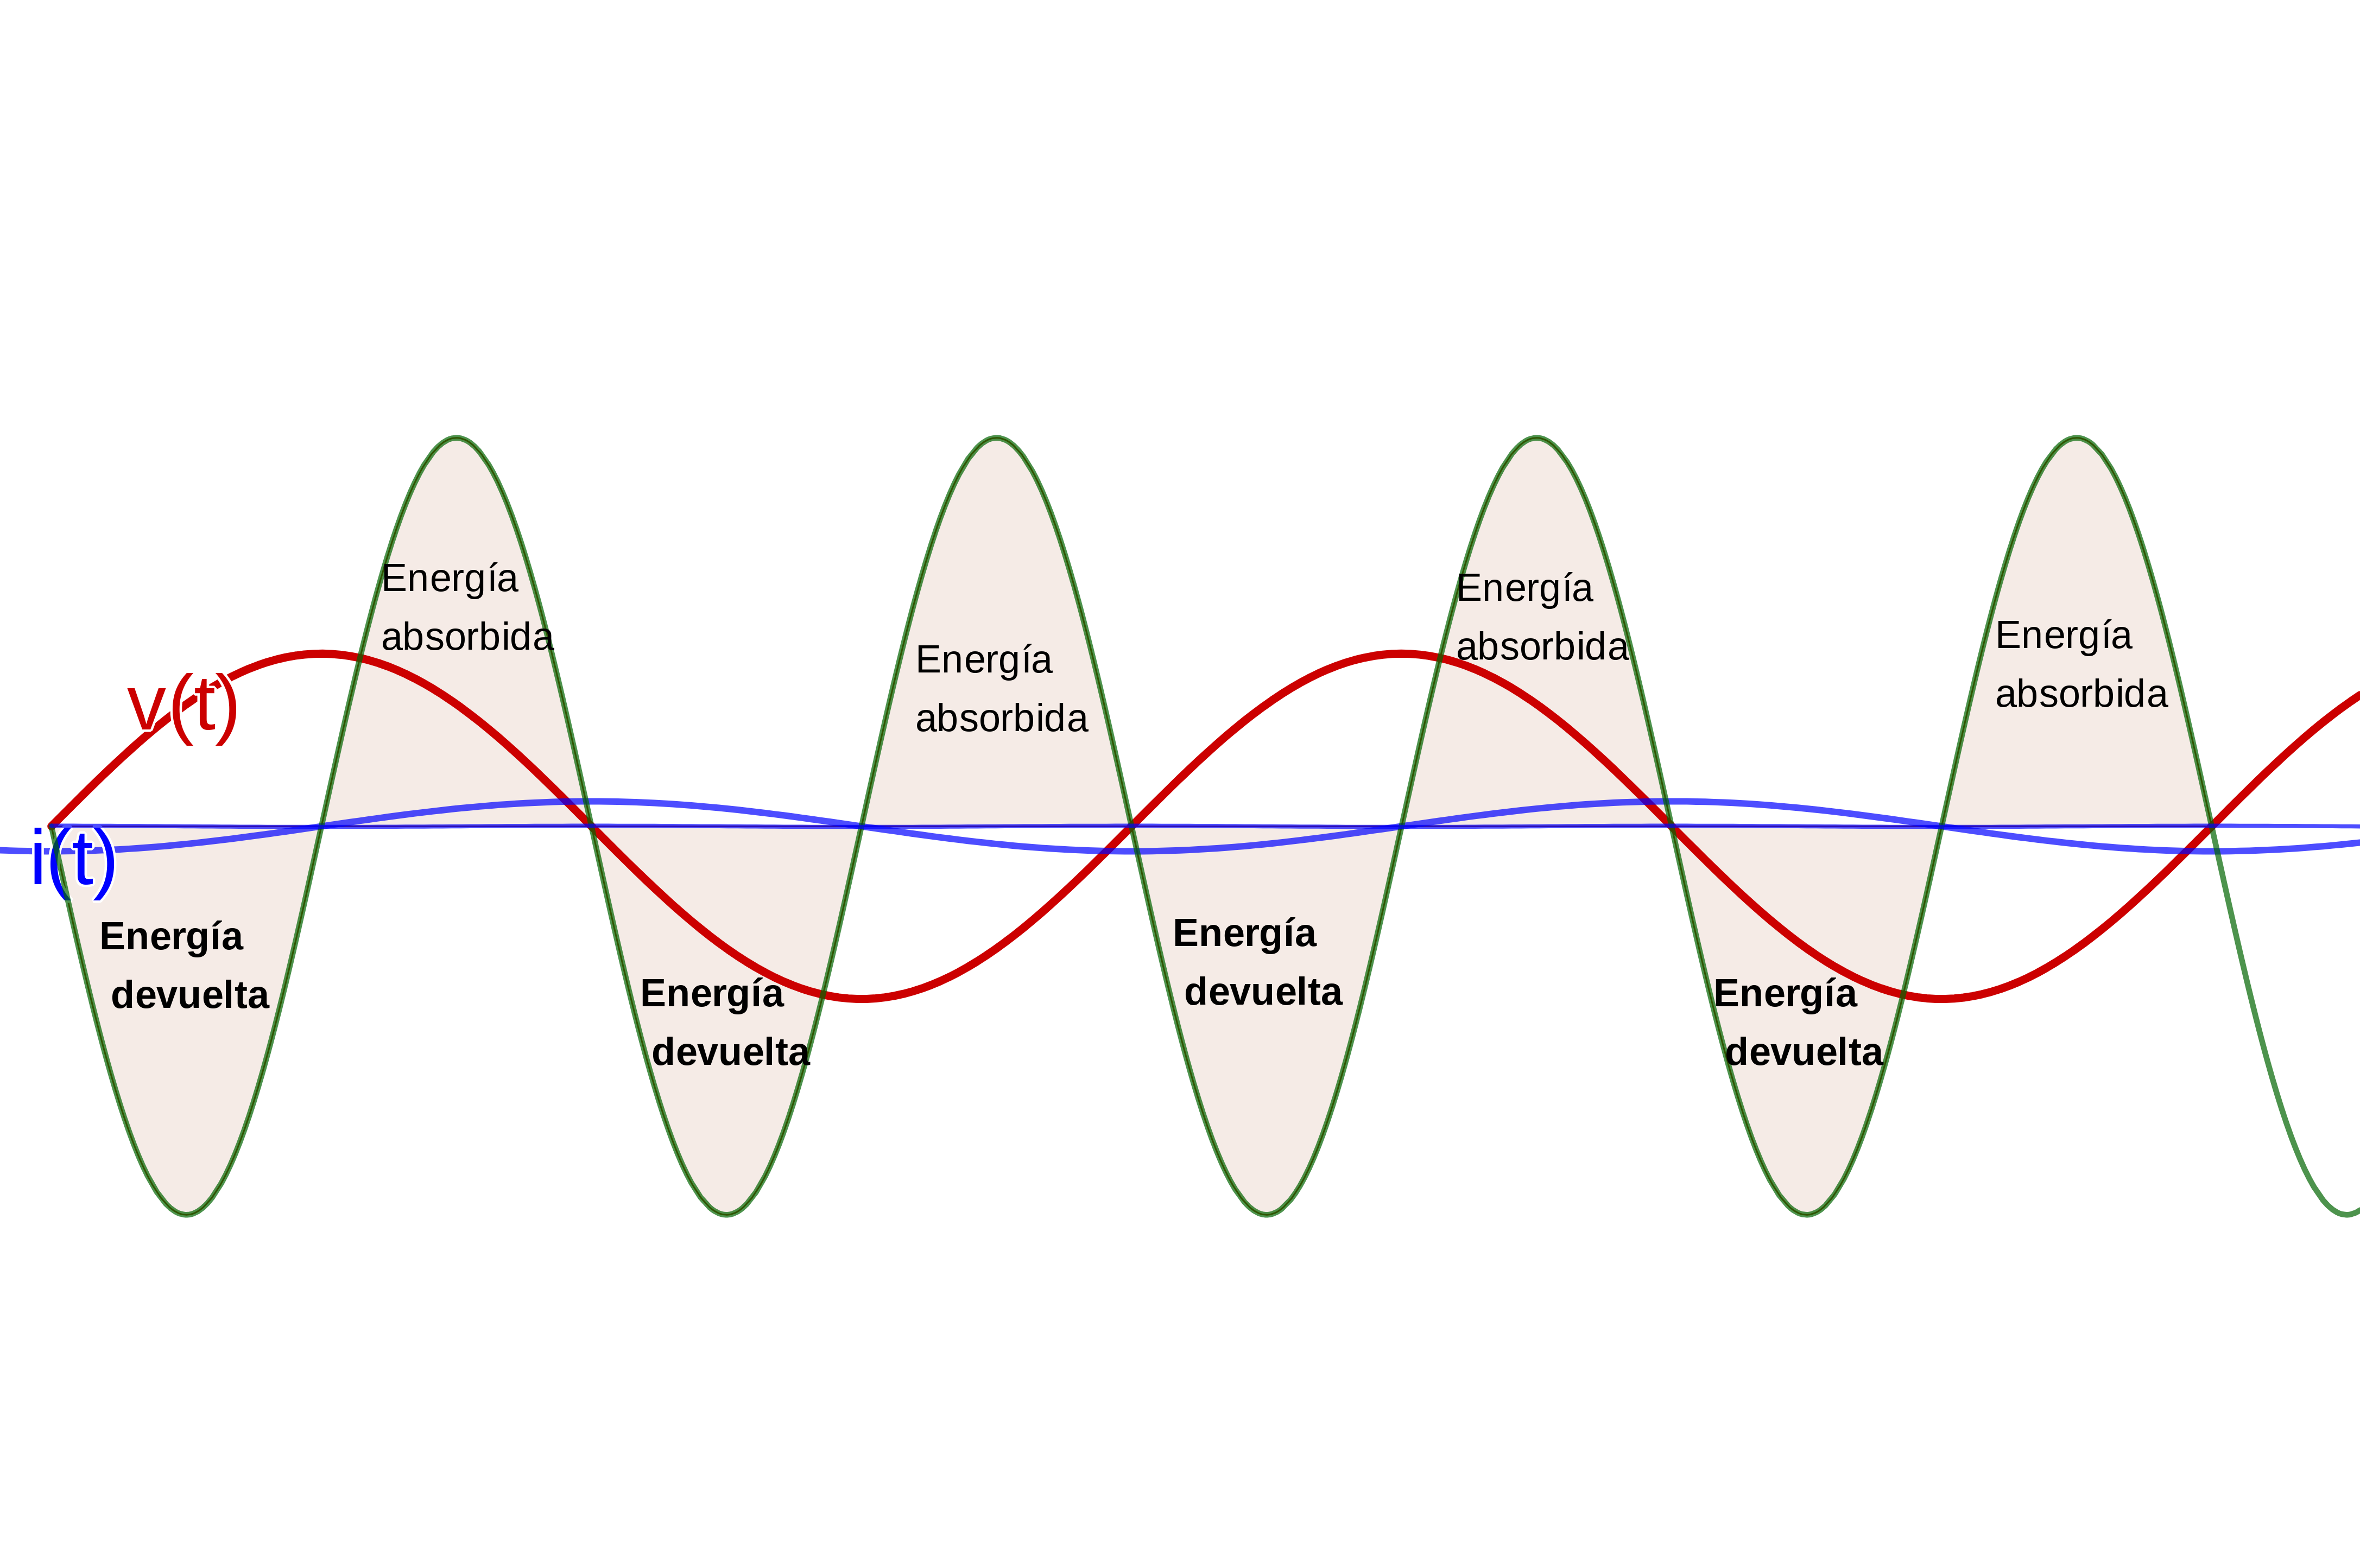
\includegraphics[scale=0.1]{images/potencia_alterna_inductiva}
  \caption{Respuesta de un circuito inductivo puro en C.A.: corriente en azul, tensión en rojo y potencia en verde}
  \label{fig:potencia_alterna_inductiva}
\end{figure}

\begin{figure}[htbp]
  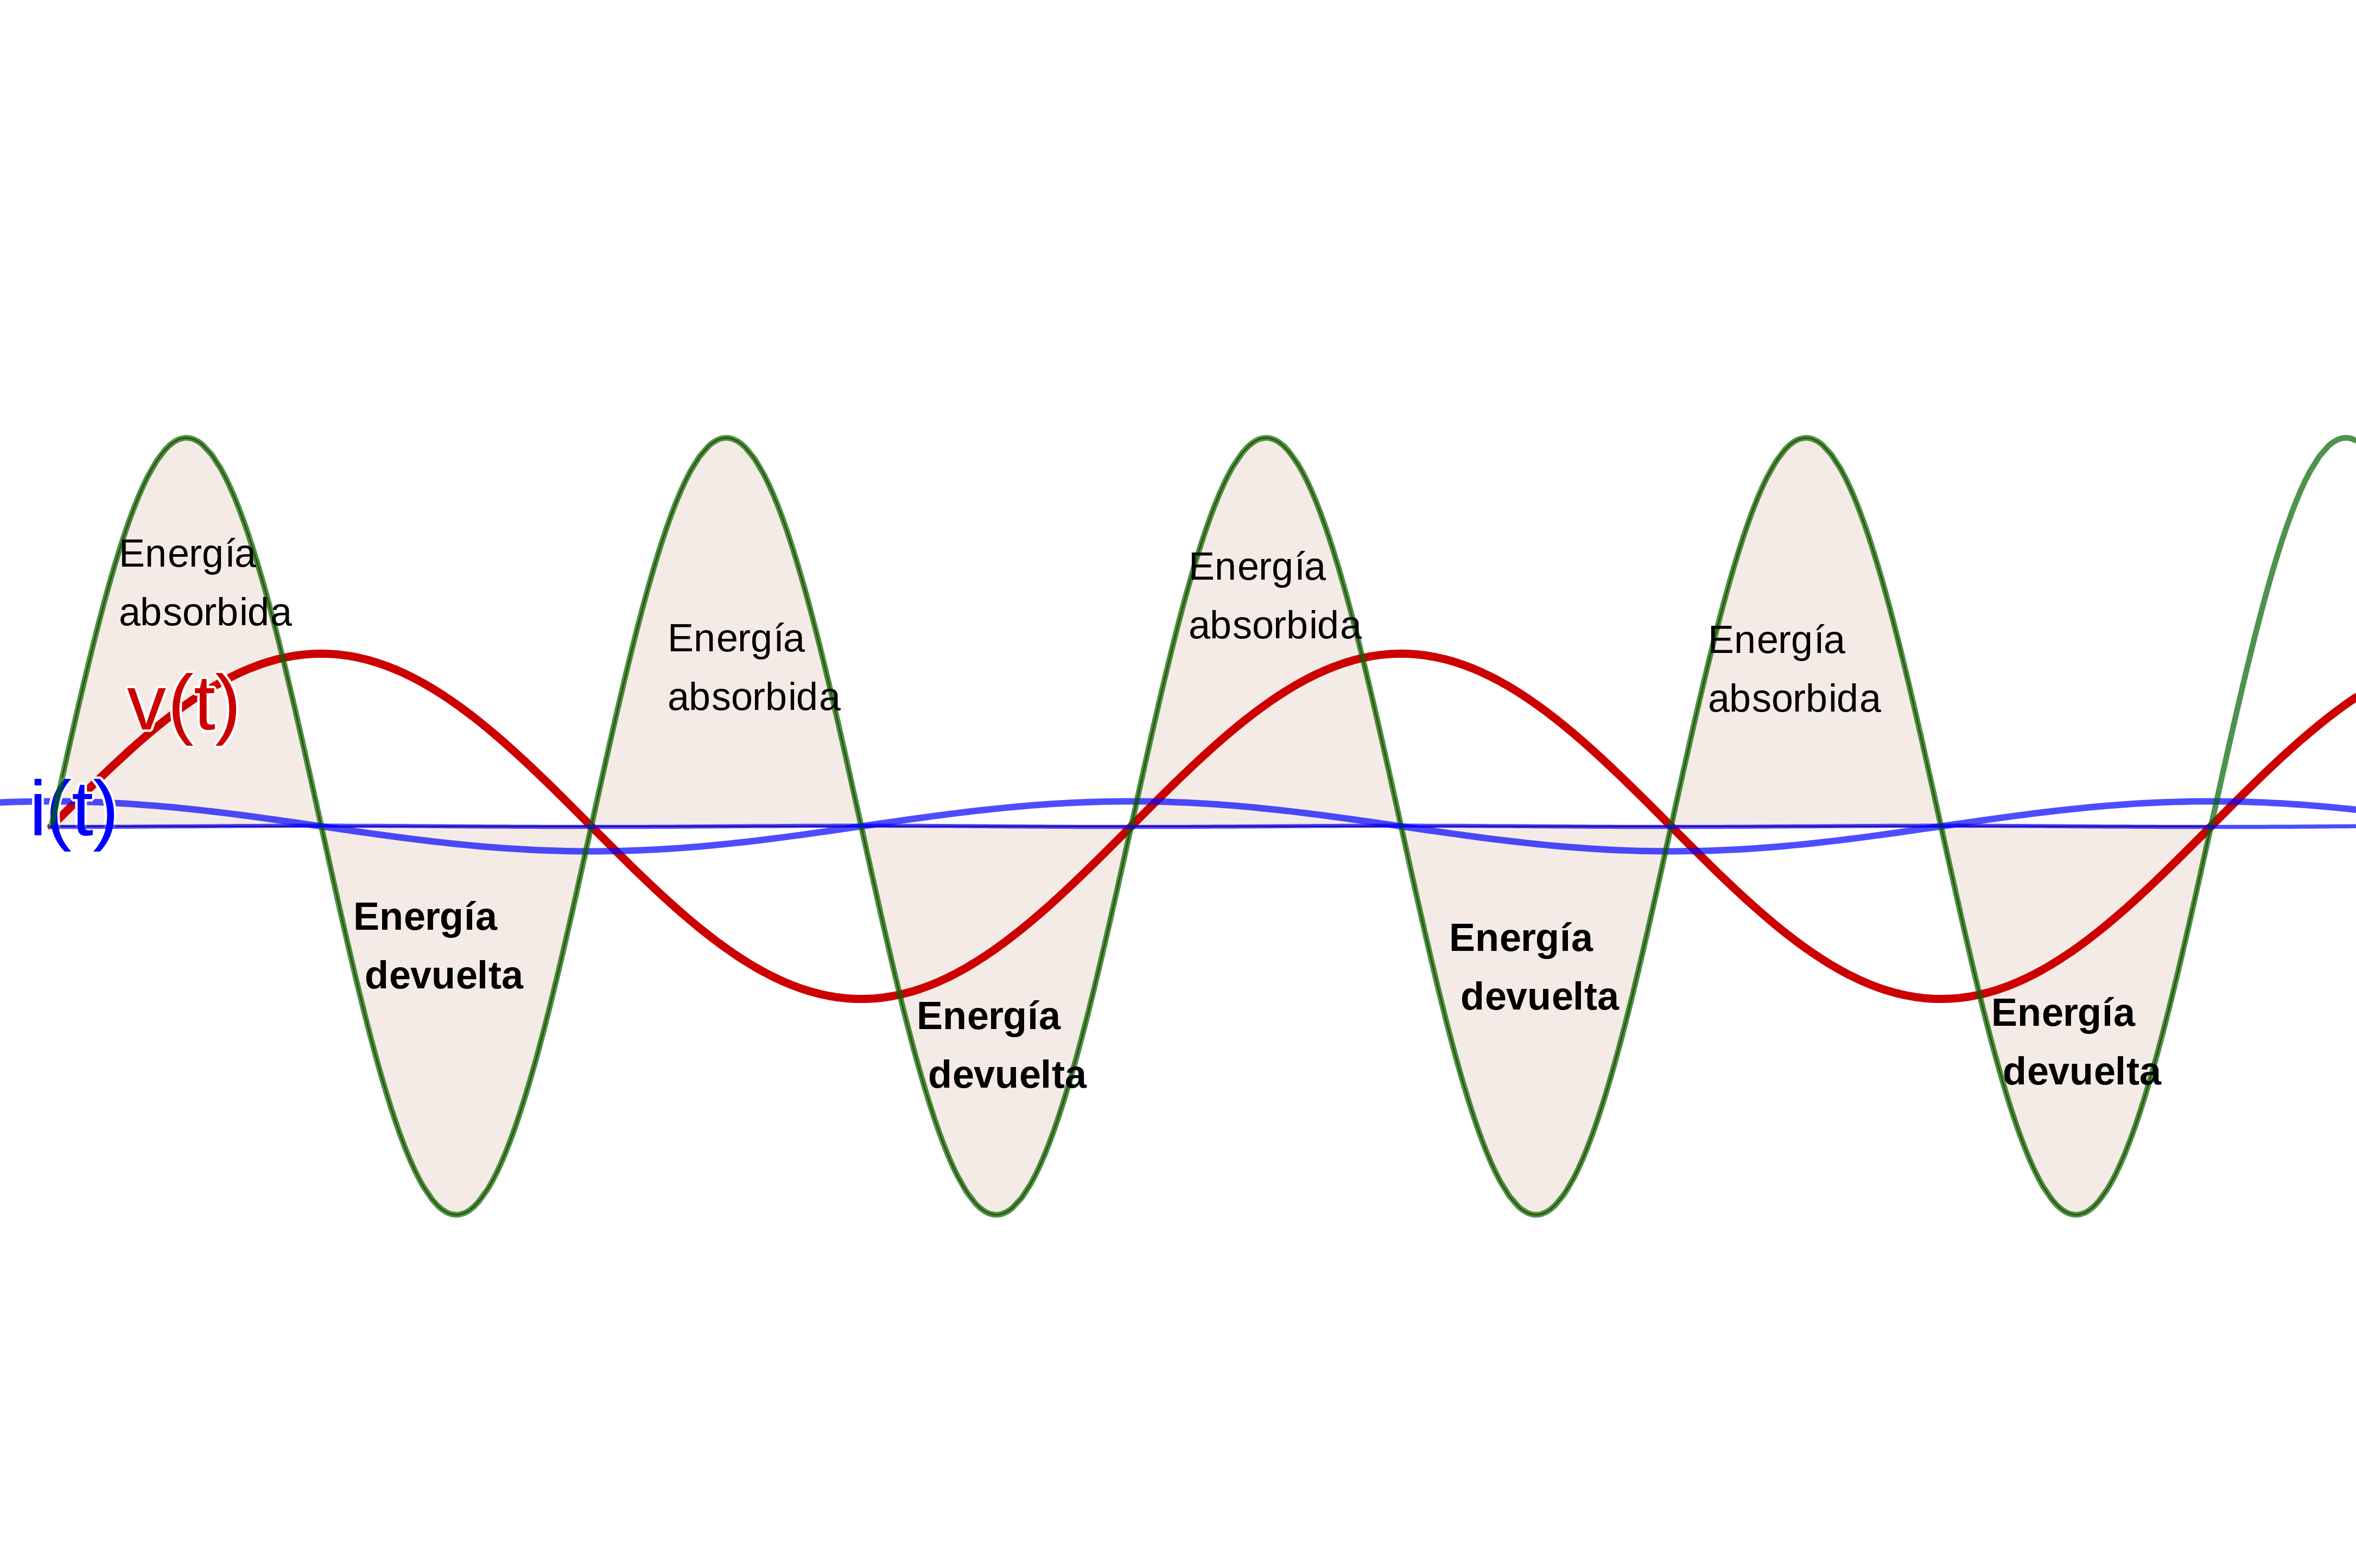
\includegraphics[scale=0.1]{images/potencia_alterna_capacitiva}
  \caption{Respuesta de un circuito capacitivo puro en C.A.: corriente en azul, tensión en rojo y potencia en verde}
  \label{fig:potencia_alterna_capacitiva}
\end{figure}

\begin{figure}[htbp]
  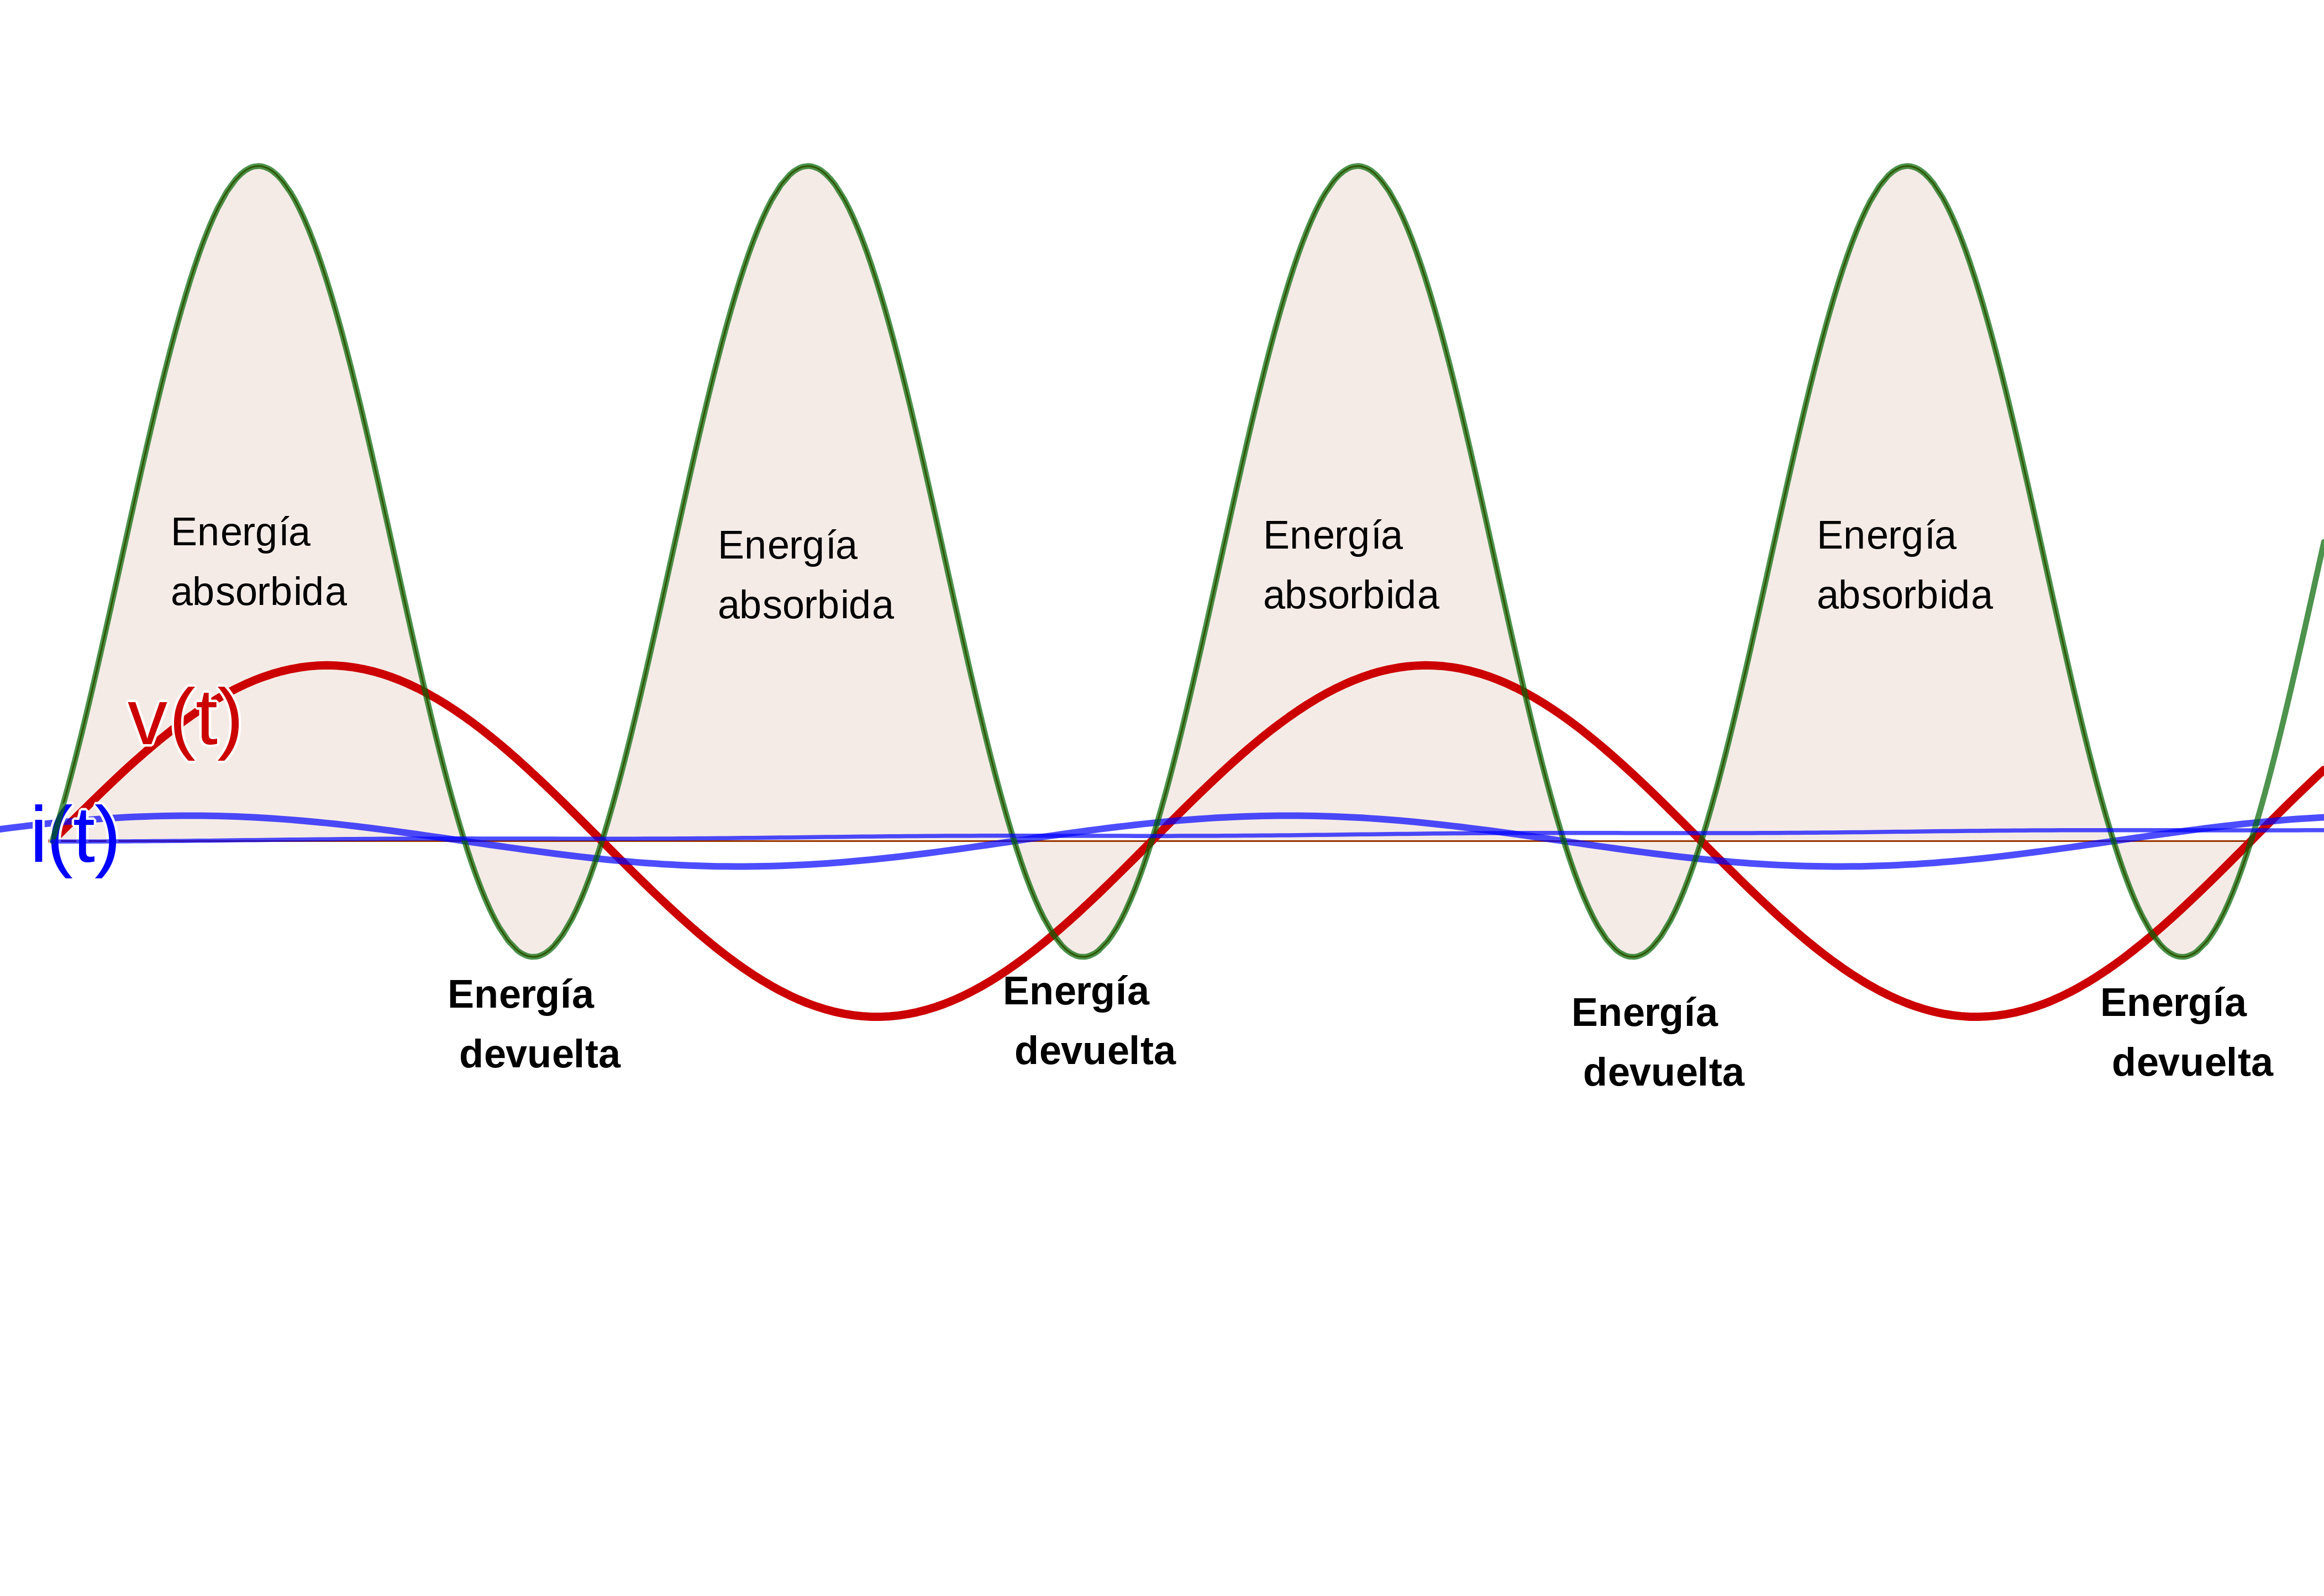
\includegraphics[scale=0.1]{images/potencia_alterna_mixta}
  \caption{Respuesta de un circuito real (resistivo y reactivo) en C.A.: corriente en azul, tensión en rojo y potencia en verde}
  \label{fig:potencia_alterna_mixta}
\end{figure}
Como la realización de operaciones con ecuaciones de ondas es algo complejo e impreciso, se verá a continuación cómo hacerlo con fasores.

\subsection{Triángulo de potencias}

Si se recuerda la representación fasorial de la impedancia, se verá que en el eje de ordenadas se expresaban los fasores de reactancia: hacia arriba $X_L$, y hacia abajo $X_C$, y en el eje de abscisas, el valor de resistencia $R$.

\begin{figure}[htbp]
  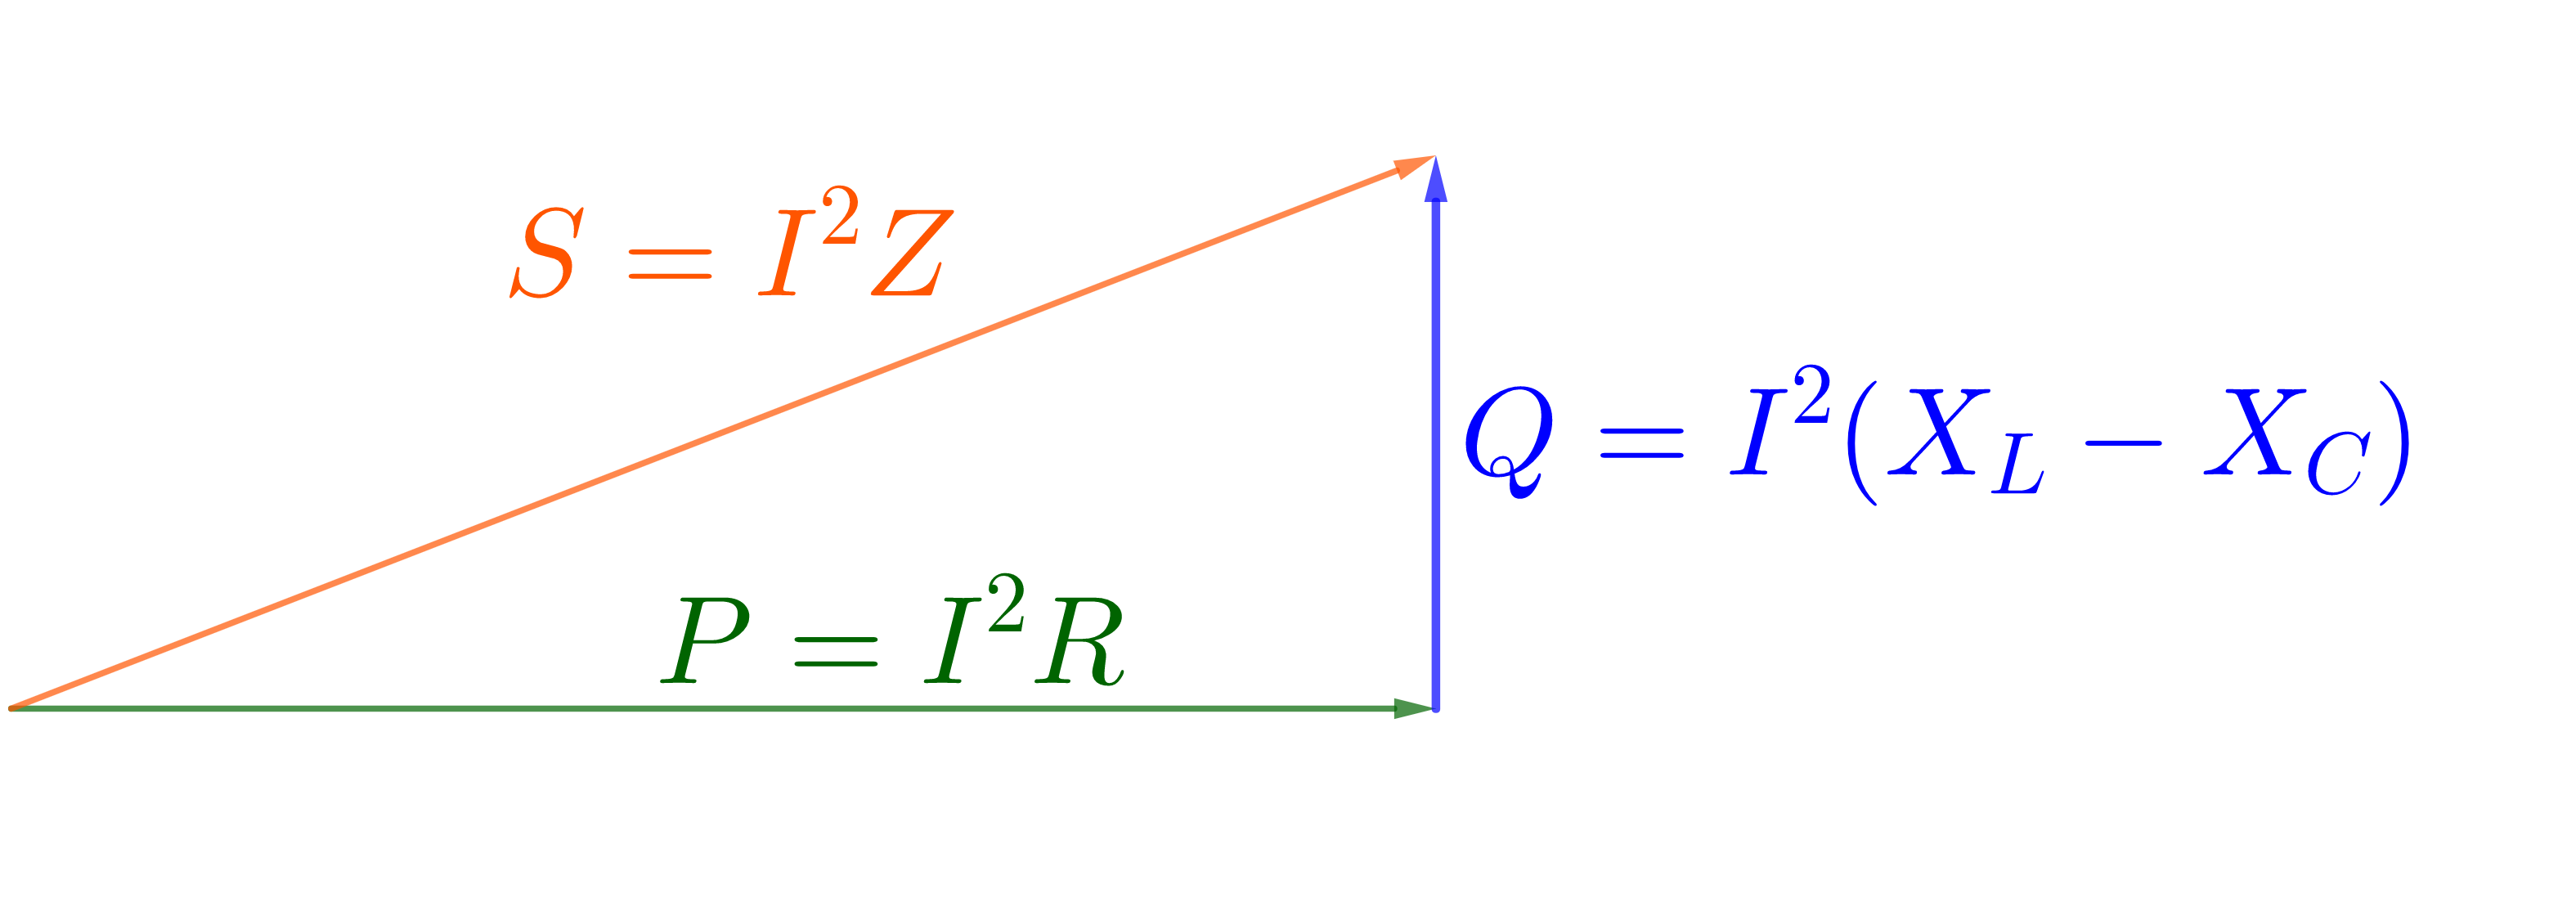
\includegraphics[scale=0.16]{images/triangulo_potencias}
  \caption{Triángulo de potencias}
  \label{fig:triangulo_potencias}
\end{figure}

El triángulo de potencias estará formado por:
\begin{itemize}
	\item La potencia activa $P$ en el eje de abscisas.
	\item La potencia reactiva $Q$ en el eje de ordenadas.
	\item La potencia aparente $S$ como la suma de ambos vectores.
	\item El ángulo entre $P$ y $S$, llamado $\varphi$.
\end{itemize}

De ese modo, la relación entre la potencia activa y la aparente es el \textbf{factor de potencia}, o también llamado \textbf{coseno de $\varphi$}, debido a que ésta es la forma en la cual se calcula.

Utilizando el Teorema de Pitágoras, se llega a la conclusión de que la relación entre las tres potencias es:

\begin{equation}
	\label{eq:potencias_alterna}
	S^{2}=P^{2}+Q^{2}
\end{equation}

Y dado que $S=V_{RMS}\times I_{RMS}$, utilizando trigonometría se pueden definir las potencias activa y reactiva como:

\begin{eqnarray}
	\label{eq:potencias_activa_reactiva}
	Q=V_{RMS}\times I_{RMS} \times sen(\varphi) \\
	S=V_{RMS}\times I_{RMS} \times cos(\varphi)
\end{eqnarray}

Como se indicó en el apartado anterior, la potencia reactiva implica el transporte de energía que no será aprovechada posteriormente. Las pérdidas en los cables por efecto Joule serán mayores aunque para el consumo efectivo de potencia activa no haya diferencias. Esto perjudica claramente a las empresas que suministran energía. Por este motivo, en talleres e industrias, se suele \textbf{penalizar el consumo reactivo excesivo}, limitando el \textbf{factor de potencia} a 0,8 (siendo 1 el valor ideal).

Por ello, suele ser necesario compensar la potencia reactiva con cargas capacitivas o inductivas.  
% \chapter{Sistemas trifásicos}

\section{Generación}

\section{Secuencias de fases}

\section{Potencia}

\section{Cargas desbalanceadas}

\chapter{Puestas a tierra}

En este capítulo se trabajará según los parámetros establecidos en el reglamento de la AEA del 2006.

Contactos directos.
Contactos indirectos.

Consideraciones del reglamento

Es indispensable, para evitar accidentes por contactos indirectos,
\begin{itemize}
	\item Sistemas de puesta a tierra.
	\item Dispositivos de corte automático.
	\item Cada masa conectada a un conductor de protección de puesta a tierra.
\end{itemize}

Existe un protocolo claro para la verificación y medición de puestas a tierra, elaborado por la Superintendencia de Riesgos de Trabajo, disponible en los recursos anexos a este documento, junto con la resolución 900 de la SRT, que regula los requerimientos de medición de puestas a tierra.

Este documento sirve para formalizar las presentaciones de los informes que se deben presentar ante ART, o SRT o las ATL (Ministerios de Trabajo Regionales de cada provincia), y se verá en profundidad cómo debe completarse en estas páginas.

Existen distintos tipos de puesta a tierra:
\begin{itemize}
	\item Toma de Tierra del neutro de Transformador.
	\item Toma de Tierra de Seguridad de las Masas.
	\item De protección de equipos electrónicos.
	\item De informática.
	\item De iluminación.
	\item De pararrayos.
	\item Otros.
\end{itemize}

Continuidad de las masas: Circuito de puesta a tierra continuo y permanente, circuito de puesta a tierra con capcaidad de conducir la carga de la corriente de falla.

Protecciones contra contactos indirectos: DD, IA, FUS.

No es lo mismo DD que ID, ya que en plantas industriales o locales comerciales grandes se requieren más de 500mA (hasta 10A) e instalaciones de hasta 2000 o 3000A de trabajo.

Interruptor automático y fusible no puede usarse en viviendas, locales comerciales (donde actúa personal no capacitado). Este tipo de instalaciones sólo puede usar esquema TT, en el cual la corriente de falla es demasiado baja como para ser vista por un IA o un FUS. Sólo se puede emplear protección diferencial de 30mA en todos los circuitos terminales y de 300mA en los circuitos principales.

No alcanza sólo con medir puestas a tierra ($R_{PAT}$), sino que en toda instalación deben actuar dispositivos automáticos de desconexión.

La creencia popular de que conectar una masa eléctrica a tierra se protege a las personas contra los contactos indirectos, ya que la tensión de contacto entre la persona y la masa sería muy baja es FALSA. La sola presencia de una puesta a tierra adecuada no asegura la seguridad de una instalación, sino que además, debe acompañarse con un dispositivo de desconexión inmediata ante la aparición de una corriente de falla. Es decir, que lo que salvará de la muerte a la persona o animal que se ponga en contacto con la masa electrificada, será la desconexión automática de la alimentación antes que se produzca el contacto.

%Este mito es completamente falso en el esquema TT (el más difundido, siendo el TN-S el  segundo más extendido y el sistema IT exclusivo para quirófanos o minas).

Las masas no se conectan en serie, sino que se debe hacer por derivación con el conductor de tierra.

%Antes de la aplicación de los reglamentos de la AEA, se solía conectar los chasis de heladeras, lavarropas y artefactos eléctricos y electrónicos a una masa aceptable, como lo era el sistema de tuberías de agua corriente (dando, la canilla metálica, una excelente puesta a tierra de bajo valor óhmico), y provocando que la corriente de defecto sea tan alta que funda el fusible, interrumpiendo el circuito. La parte fundamental de esto es que EL FUSIBLE SE FUNDE Y DESCONECTA EL CIRCUITO, ya que de producirse el contacto humano con el chasis electrificado, la persona recibiría la descarga, de no ser por la interrupción del circuito provocada por el fusible.

El problema de los electrodos dispersos: si existen electrodos dispersos en la instalación eléctrica, la puesta a tierra no es aceptable, debido a que no existe equipotencialidad.

CIRCUITOS TERMINALES DE HASTA 32A

El tiempo de desconexión depende del ECT y del tipo de circuito que se utilice.
Cualquiera sea el ECT adoptado, si el circuito terminal tiene un consumo de hasta $32\; A$ para las tensiones de servicio ($220\; V$), la protección contra C.I. debe realizarse en los tiempos máximos siguientes:

\begin{itemize}
	\item Esquema TN-S: $0,2\; s=200\; mS$.
	\item Esquema TT: $0,06\; s=60\; mS$.
\end{itemize} 

Para los esquemas TT, se deben utilizar los DD de $30\; mA$, pero para verificar la seguridad, se debe utilizar los tiempos de disparo recorridos por \textbf{5 veces la corriente diferencial}. Entonces es falso que \textbf{los diferenciales deban actuar en $30\; mS$}

Las $R_{PAT}$ no necesitan ser tan bajas como se cree.

La resolución 900 pide que se realice una verificación anual de las puestas a tierra, y que los telurímetros utilizados tengan una certificación (sin importar su antigüedad).

Ensayos para verificar si el dispositivo diferencial puede desconectar ante contactos indirectos indicados por la norma:
\begin{enumerate}
	\item Un diferencial no debe disparar con la mitad de la corriente diferencial (un diferencial de $30\; mA$ no debería dispararse con una corriente de $15\; mA$ o menos).
	\item Se debe aplicar la corriente de $30\; mA$ en una sola aplicación y el diferencial deberá disparar en un tiempo no mayor a $300\; mS$.
	\item Si el diferencial está recorrido por el doble de su corriente diferencial, el dispositivo deberá dispararse en la mitad del tiempo máximo. Es decir, que si a un diferencial de $30\; mA$ se le aplican $60\; mA$, deberá disparar en un tiempo no mayor a $150\; mS$.
	\item Se debe comprobar el tiempo de disparo al aplicar 5 veces su corriente nominal, y deberá ser como máximo de $40\; mS$.
\end{enumerate}

Cuando se emplea protección diferencial no se debe considerar el tiempo de apertura $I_{\Delta n}$ sino $I_{\Delta n}$.

CIRCUITOS SECCIONALES O MAYORES A 32A

Para circuitos seccionales (aquellos que van de tablero a tablero) o para circuitos terminales mayores a $32\; A$), se permitirán tiempos mayores a los mencionados anteriormente, permitiendo aplicar el principio de selectividad.

Para el esquema TN-S, se admitirán tiempos de desconexión de hasta 5 segundos, mientras que para el esquema TT, el tiempo máximo de desconexión será de 1 segundo.

USO DEL CRITERIO DE SELECTIVIDAD
\begin{ejemplo}
	En una vivienda, se utiliza un interruptor diferencial de $100\; mS$ selectivo en el tablero principal. Este tablero se conecta con otros tres tableros terminales diferentes, siguiendo la siguiente regla de seccionamiento:
	\begin{enumerate}
		\item Cocina, baño.
		\item Habitación 1, habitación 2.
		\item Patio, cochera.
	\end{enumerate}
 	En cada tablero terminal, se utilizan interruptores de $30\; mA$.
 	
 	Al producirse una falla en la aislación de un velador de la habitación 2, actúa el interruptor diferencial del tablero 2, permitiendo reconocer la falla de manera más sencilla y sin dejar sin alimentación al resto de la vivienda.
\end{ejemplo}

%Inst q mida corrientes de corto, corrientes de falla, imp en lazos de falla, funcionamiento de los diferenciales.

ELECTRODOS DISPERSOS

Es común observar, en distintas instalaciones, electrodos dispersos (en distintas máquinas, al pie de una central telefónica, al pie de equipos de telecomunicaciones, etc.)

Esto está prohibido por el reglamento, a menos que estos electrodos se conecten entre sí y a la barra de puesta a tierra, logrando equipotencializarse.

Las masas eléctricas y las masas extrañas deben conectarse a un conductor de equipotencialidad o en su defecto, al conductor de protección.

Conductor de equipotencialidad y conductor de protección: ...

Los electrodos de puesta a tierra de descargas atmosféricas deben estar conectados a la barra de cobre de puesta a tierra del tablero principal. Esto evitará la aparición de arcos eléctricos porque habrá equipotencialidad entre las masas de tierra y del edificio o instalación.

%Normas en otros países IE32605 AEA32605 FPA780 NVR519

ESQUEMAS DE CONEXIÓN A TIERRA

Para establecer las condiciones de protección (tensiones de contacto esperables y tiempos máximos tolerables de desconexión) es necesario conocer el esquema de conexión a tierra empleado.
 
ESQUEMA TT

\begin{figure}[htbp]
  \centering  
  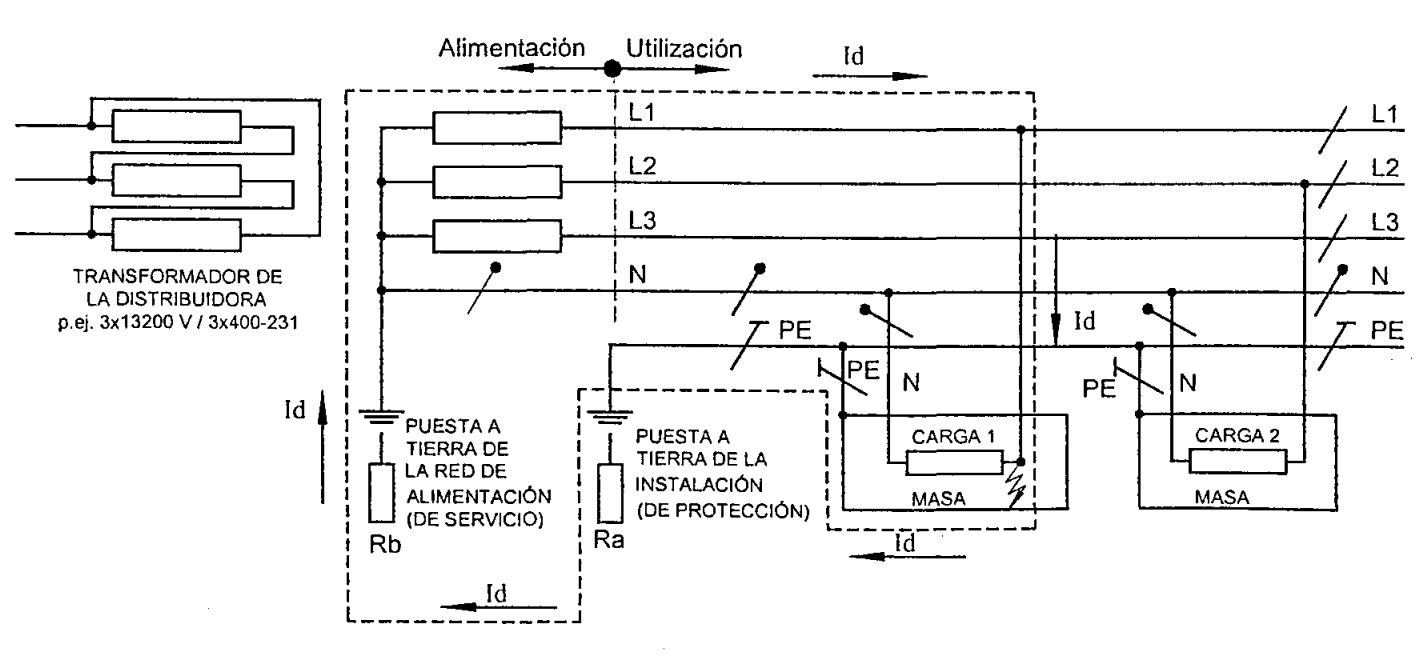
\includegraphics[width=\textwidth]{images/ect-tt}
  \caption{ECT TT. Fuente: AEA, 2006}
  \label{fig:ect-tt}
\end{figure}

En el esquema se puede apreciar la puesta a tierra de servicio $R_b$, la puesta a tierra de protección $R_a$, los conductores de puesta a tierra $PE$ conectados desde el electrodo $R_a$ a la \textbf{barra de puesta a tierra $PE$}, y a todos los tomacorrientes de tres espigas.
Al producirse un contacto indirecto, la corriente de defecto $I_d$ circulará desde la fase $L_1$ hasta el electrodo $R_a$, para luego recorrer por tierra la distancia que sea necesaria hasta alcanzar el electrodo de puesta a tierra de servicio $R_b$ y cerrar el circuito.

El valor de resistencia de puesta a tierra puede, según el reglamento, alcanzar los $40\; \Omega$ siempre y cuando la protección diferencial posea una corriente de disparo máxima de $300\; mA$.

\begin{ejemplo}
	Dada una puesta a tierra en un buen suelo, en el que se ha alcanzado una resistencia de puesta a tierra de $10\; \Omega$, y la distribuidora de energía posee una resistencia de puesta de servicio de $1\; \Omega$, la corriente de defecto se podría calcular según la Ley de Ohm, de la siguiente forma:
	
	$$I_d= \frac{V_{\text{línea}}}{\text{Suma de resistencias}}$$
	$$I_d = \frac{220\; V}{10\; \Omega + 1\; \Omega}=20\; A $$

	Es decir que ante una falla en una instalación típica, un valor de corriente cercano a $20\; A$ circulará por la rama de la corriente de defecto. Este valor es muy superior a los valores de corte de los interruptores diferenciales.
\end{ejemplo}

Las siglas TT indican Tierra-Tierra. Esto significa que el sistema dispone de una puesta a tierra de servicio y una puesta a tierra para la instalación por separado. La puesta a tierra de servicio es responsabilidad de la empresa distribuidora, mientras que la tierra de la instalación es trabajo del instalador.

Nunca se debe, en un esquema TT, conectar la tierra con neutro, debido a que la seguridad dependería de la calidad del neutro que entregue la compañía. Además, esto provocaría que el esquema se convierta en TN-S.

La Ley fija que la tensión de contacto máxima es de $24\; V$, y toda tensión superior en masas eléctricas o extrañas, deberá ser detectada por el diferencial e interrumpida de inmediato para evitar accidentes.

El protocolo exige medir $R_a$ (el cual deberá ser menor a $40\; \Omega$, verificar la continuidad de los conductores de protección (aquellos que van desde cada dispositivo y tomacorriente de tres contactos al conductor de tierra) y del conductor de tierra (que es el conductor que va desde el electrodo $R_a$ hasta la barra de puesta a tierra en el tablero principal. Se deberá verificar también, mediante los distintos ensayos, el dispositivo de protección que proteja contra contactos indirectos (interruptor diferencial). 

TN-S
%Imagen

Las instalaciones que utilizan este esquema son aquellos que toman en media tensión (como por ejemplo grandes industrias) o aquellos que han incorporado un transformador en su instalación, con el fin de adecuar el sistema a TN-S (por venir de un ECT TT).

Aquí el conductor de protección de la instalación se conecta a la barra de neutro. De ahí el nombre TN (Tierra-Neutro).

Por otra parte, se debe destacar que la conexión entre tierra y neutro se hace en las barras del tablero principal, pero los conductores de tierra y de neutro deberán estar separados a lo largo de la instalación (por ello la letra S en TN-S).

La corriente de falla se produce por los elementos metálicos (no por la tierra) y por ello es de muy alto valor y se permite utilizar fusibles o interruptores automáticos (además de diferenciales, como era el caso del esquema TT).

Dicho de otra forma, la resistencia $R_b$ no participa del lazo de corriente de falla, pero aún así debe poseer un valor muy bajo por otras razones: ... ESCRIBIR RAZONES



TN-C
IT
\chapter{Instrumentos de medición}

Incluir cómo afecta a las mediciones la variación de la Temperatura.
\section{Multímetro}
\subsection{Voltímetro}
\subsection{Amperímetro}
\subsection{Óhmetro}
\section{Vatímetro}
\section{Capacímetro}
\section{Frecuencímetro}
\section{Pinza amperométrica}
\section{Megóhmetro}
\section{Telurímetro}
\section{Osciloscopio}
\section{Comprobadores de tensión}
\subsection{Buscapolo}
\subsection{Medidor inductivo}
\section{Cofímetro}
\section{Medidor de energía}
\section{Medidor de campo electromagnético}
\chapter{Máquinas eléctricas}
En este capítulo se desarrolla una explicación general acerca de los tres grandes tipos de máquinas eléctricas.

Se explicarán los principios de funcionamiento y se analizarán algunas ecuaciones que serán de ayuda para realizar ensayos durante este curso. Debe tenerse en cuenta que el estudio de máquinas eléctricas requiere de un curso por sí mismo (como mínimo), por lo que el estudio que se realizará aquí, no es para nada exhaustivo.

\section{Transformadores}

Un transformador es una máquina eléctrica que cuenta con dos devanados concatenados mediante un circuito eléctrico de alta permeabilidad magnética. Existirá un flujo magnético que inducirá una fuerza electromotriz entre sus devanados, relacionados por el número de espiras entre ambas.
\begin{equation}
	\label{eq:relacion_espiras_transformador}
	\frac{N_1}{N_2}=\frac{V_1}{V_2}
\end{equation}
Siendo $N_1$ y $N_2$ el número de espiras de los devanados primario y secundario respectivamente, y $V_1$ y $V_2$ los valores de tensión eficaz obtenidos en cada uno de los devanados.
\section{Generadores}
\section{Motores}

\chapter{Prácticas de laboratorio}

\section{Mediciones en CC}
\subsection{Prueba de componentes}
Diodos, fusibles, resistencias, inductancias, capacitores.
\section{Ensayos sobre instalaciones de CA}
\subsection{Consumos}
\subsection{Energía}
\subsection{Puesta a tierra}
\subsection{Potencia}
activa, reactiva, aparente, factor de potencia.
\subsection{Armónicas}
Lámparas de distinto tipo, cargas de distinto tipo, fuente de PC, fluorescente, led, etc..

\section{Ensayos sobre máquinas eléctricas}
\subsection{Motores de CA}
\subsubsection{Aislamiento}
\subsubsection{Bobinados}
\subsubsection{Frecuencia}
\subsection{Transformadores}
	\subsubsection{Transformador de aislación galvánica}
	Usando el gabinete de pruebas...
\section{Tratamiento digital de datos}
\begin{thebibliography}{X}
	% \bibitem{Ref2} \textsc{Autores}, (AÑO). \textit{Título}, ciudad, editorial.	
	\bibitem{boylestad} \textsc{Boylestad, R.}, (2011). \textit{Introducción al análisis de circuitos} Decimosegunda edición, México, Pearson Educación.
	\bibitem{hewitt} \textsc{Hewitt, P.} (2002). \textit{Conceptual physics}. Pearson Educación.
	\bibitem{bolton} \textsc{Bolton, W.} (1995). \textit{Mediciones y pruebas eléctricas y electrónicas}. Marcombo.
	\bibitem{uniandes} \textsc{Calderón, J.} (2006). \textit{Fundamentos de las Mediciones Eléctricas. Teorı́a y Prácticas de Laboratorio}. Escuela de Ingenierı́a Eléctrica, Universidad de Los Andes.
	\bibitem{utnmendoza} \textsc{Samsó, F.} (2008). \textit{Apuntes de Cátedra de Máquinas e Instalaciones Eléctricas}. Departamento de Electŕonica. Universidad Tecnológica Nacional: Facultad Regional Mendoza.
	\bibitem{maqelec} \textsc{Ortega, G.; Gómez, M. \& Bachiller, A.} (2002). \textit{Problemas Resueltos de Máquinas Eléctricas}. Thomson. Madrid.
	\bibitem{suarez} \textsc{Suárez, J. A.} (2006). \textit{Medidas Eléctricas: segunda edición}. Libro de cátedra de Mediciones Eléctricas I: Facultad de Ingeniería, Universidad Nacional de Mar del Plata.
	\bibitem{frank} \textsc{Frank, E.} (1969). \textit{Análisis de Medidas Eléctricas}. McGraw Hill. Madrid.
	\bibitem{aeabt} \textsc{Asociación Electrotécnica Argentina} (2007). \textit{Documento Normativo 95150. Suministro y medición en baja tensión}. AEA.
	\bibitem{aeamantenimiento} \textsc{Asociación Electrotécnica Argentina} (2006). \textit{Documento Normativo 90706 Guía para la gestión del Mantenimiento en instalaciones. }. AEA.
	\bibitem{aeamantenimiento} \textsc{Asociación Electrotécnica Argentina} (2006). \textit{Documento Normativo 90364-7-771 Reglamentación para la ejecución de instalaciones eléctricas en inmuebles – Viviendas, oficinas y locales (unitarios). }. AEA.
	%Materiales del curso de EDx
	
\end{thebibliography}

%\chapter{Introdução}

\thispagestyle{empty} 

Este modelo tem como base as instruções da Editora UnB para a editoração dos livros da série \textit{Ensino de Graduação}. Autores de ciências naturais ou exatas gostam de usar \LaTeX, sistema de editoração que não é muito por editoras dedicadas às humanidades. Dá um certo trabalho adequar um livro às regras da ABNT em \LaTeX. Espero que este modelo encoraje outras pessoas a submeterem seus livros à Editora UnB.

\begin{mdframed}[style=noteSty]

{\center \textsc{Texto motivador} \par}

   Este é um breve texto motivador. Espero que você esteja motivado(a)!
   
\end{mdframed}

Muitos cientistas gostam de usar \LaTeX porque essa ferramenta possibilita escrever facilmente equações como a seguinte:
\begin{equation}
 \mathscr{p}+\frac{1}{2}{\rho}v^2+{\rho}gh = \text{constante}
 \label{eq:Bernoulli}
\end{equation}
onde $\mathscr{p}$ é a pressão, $v$ é a velocidade e $h$ é a elevação, ou seja, a “altura do tubo”. Essa equação pode ser deduzida a partir do \textit{Teorema Trabalho-Energia}. \index{Teorema Trabalho-Energia}  % entrada para o índice remissivo

\newpage

Note como a numeração das páginas começa aqui.
%\cleardoublepage

%\chapter{Figuras e gráficos}

\thispagestyle{empty} 

Sugiro que você guarde todas as figuras na pasta ``figs'' para que seu projeto fique mais organizado. A figura \ref{fig:logolatex} mostra como é fácil inserir uma figura com legenda e referência à fonte.

\begin{figure}
	\centering
	\begin{minipage}{0.6\linewidth}
		\centering
		\caption{Logo \LaTeX.}
		\label{fig:logolatex}
		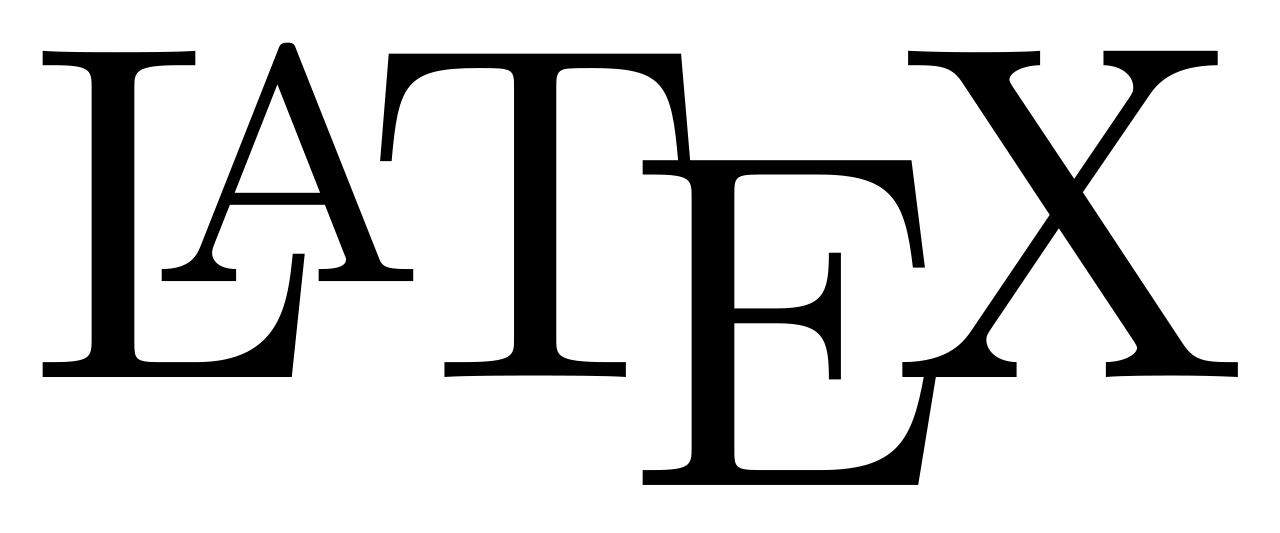
\includegraphics[width=\linewidth]{figs/1280px-LaTeX-logo.png}
		\source{Wikimedia Commons \cite{wikimedia-latex}.}
	\end{minipage}
\end{figure}

Além de figuras, \index{figuras} é possível inserir caixas de texto de diversos tipos, como axiomas, teoremas etc. Elas podem ser configuradas e novos tipos delas podem ser criados no arquivo \begin{verbatim}config/envs.tex\end{verbatim}.

Existem pacotes que permitem criar figuras e gráficos no próprio código \LaTeX. Por exemplo, temos

\begin{itemize}
    \item PGFPlots \url{http://pgfplots.sourceforge.net/}
    \item TikZ \url{http://www.texample.net/tikz/examples/all/}
    \item Metapost \url{http://tex.loria.fr/prod-graph/zoonekynd/metapost/metapost.html}
    \item PSTricks \url{https://tug.org/PSTricks/main.cgi?file=examples}
\end{itemize}

\begin{question}
    Explique como Isaac Newton usaria cada um dos pacotes seguintes, se vivesse no tempo presente:
    \begin{enumerate}[label=(\Alph*)]
        \item Metapost
        \item TikZ
        \item PGFPlots
        \item PSTricks
    \end{enumerate}
\end{question}

\begin{solution}
    \begin{enumerate}[label=(\Alph*)]
        \item Para fazer figuras 3D.
        \item Para fazer diagramas.
        \item Para traçar gráficos.
        \item Para fazer de um tudo.
    \end{enumerate}
\end{solution}

\section{Soluções deste capítulo}

\printsolutions
%\clearpage
%%\fancyfoot[CO,CE]{}
\fancyfoot[LO]{\small}
\fancyfoot[RO]{\small}
%\fancyfoot[CE]{\Author}
\fancyfoot[LE]{\small}
\fancyfoot[RE]{\small}

\begin{discussion}

\hfill

\begin{center}
  \textsc{\large Criando quadros}\\
\end{center}

\vspace{1ex}

\begin{flushright}
  \textbf{Leonardo Luiz e Castro} \\
  \vspace{1ex}
  \textit{\small Instituto de Física} \\
  \textit{\small Universidade de Brasília} \\
\end{flushright}

\addcontentsline{toc}{section}{Texto complementar -   Criando quadros (Leonardo Luiz e Castro)}

\vspace{1ex}

\section*{O que são quadros?}

Quadros são parecidos com tabelas, com a diferença de que não contêm dados numéricos, mas sim informação textual. Aparentemente, a ABNT é pioneira no mundo em se preocupar com tal distinção.

\section*{Exemplo de quadro em \LaTeX?}

Preferi listar os quadros como figuras. Vi algum livro que fazia assim... Veja como a figura \ref{fig:estados-da-materia} ficou interessante! Lembre-se que só é possível inserir uma figura dentro de um ambiente como este se a opção de não flutuação ([H]) for utilizada.

\begin{figure}[H]
	\centering
	\begin{minipage}{\hsize}
		\centering
		\taburulecolor{white}\arrayrulecolor{white}
		\caption{Quadro de caracterização dos estados da matéria.}
		\label{fig:estados-da-materia}
		\begin{tabular}{| >{\centering\cellcolor{verde_UnB}\color{white}}p{0.11\hsize} | >{\centering\cellcolor{verde_UnB}\color{white}}p{0.12\hsize} | >{\centering\cellcolor{verde_UnB}\color{white}}p{0.12\hsize} | >{\centering\cellcolor{verde_UnB}\color{white}\footnotesize}p{0.11\hsize} | >{\centering\cellcolor{verde_UnB}\color{white}\footnotesize}p{0.16\hsize} | >{\centering\cellcolor{verde_UnB}\color{white}\footnotesize}p{0.17\hsize} |}
			\hline
			{\bf Estado} & {\bf Volume} & {\bf Forma} & {\bf É fluido?} & {\bf É matéria condensada?} & {\bf É compressível?} \tabularnewline
			\hline
		\end{tabular}
		\begin{tabular}{| >{\centering\cellcolor{verde_UnB!70}\color{white}\small}p{0.11\hsize} | >{\centering\cellcolor{verde_UnB!50}\color{black}\small}p{0.12\hsize} | >{\centering\cellcolor{verde_UnB!50}\color{black}\small}p{0.12\hsize} | >{\centering\cellcolor{verde_UnB!50}\color{black}\small}p{0.11\hsize} | >{\centering\cellcolor{verde_UnB!50}\color{black}\small}p{0.16\hsize} | >{\centering\cellcolor{verde_UnB!50}\color{black}\small}p{0.17\hsize} |}
			\hline
			Gasoso & ajustável & ajustável & sim & não & muito \tabularnewline
			\hline
			Líquido & fixo & ajustável & sim & sim & pouco \tabularnewline
			\hline
			Sólido & fixo & fixa & não & sim & não \tabularnewline
			\hline
		\end{tabular}
		\source{elaboração do autores de Física para Ciências Agrárias e Ambientais (Leonardo Castro e Olavo Filho).}
	\end{minipage}
\end{figure}

\end{discussion}

%\cleardoublepage

%\chapter{Ambientes}

\thispagestyle{empty}

Este modelo disponibiliza alguns ``ambientes'', ou seja, caixas de texto com formatação especial para certos tipos de elementos que são automaticamente numerados (e.g. teorema 1.1, teorema 1.2 etc.). Ambientes podem ser criados e configurados por edição do arquivo envs.tex da pasta config.

\section{Exemplos de ambientes disponíveis}

\begin{axiom}
    \LaTeX produz equações mais bonitas que qualquer editor WYSIWYG.
\end{axiom}

\begin{theorem}\textsc{teorema LaTeX-WYSIWYG}
    Todo físico prefere usar código \LaTeX puro que qualquer editor WYSIWYG.
\end{theorem}

\index{\LaTeX} % entrada para o índice remissivo
\index{WYSIWYG}

\begin{demonstration}
    Físicos gostam de equações bonitas. Editores What-You-See-Is-What-You-Get não são apropriados para fazer equações bonitas.\footnote{É certo que há editores WYSIWYG baseados em \LaTeX, mas eles não nos dão o mesmo nível de controle.} Logo, se algum físico preferisse usar um editor WYSIWYG no lugar de \LaTeX, não seria muito inteligente. Como todo físico é inteligente, o teorema está demonstrado \textit{ad absurdum}.
\end{demonstration}

\begin{example}
    Einstein usaria um editor WYSIWYG ou \LaTeX? \\
    Einstein era físico. Portanto, usando o teorema LaTeX-WYSIWYG, concluímos que ele usaria \LaTeX.
\end{example}

\begin{question}
    Einstein usaria um editor WYSIWYG ou \LaTeX?
\end{question}

\begin{solution}
    Einstein era físico. Portanto, usando o teorema LaTeX-WYSIWYG, concluímos que ele usaria \LaTeX.
\end{solution}

\begin{question}
    Marie Curie usaria um editor WYSIWYG ou \LaTeX?
\end{question}

\begin{solution}
    Deixamos esta sem resposta para o estudante se esforçar mais.
\end{solution}

\clearpage

\section{Soluções deste capítulo}

\printsolutions
%\cleardoublepage

%\chapter{Conclusão}

\thispagestyle{empty}

Você deve começar a editar o seu livro agora mesmo!
%\cleardoublepage


% Apêndices:

\renewcommand\appendixname{ANEXOS}
\renewcommand\appendixpagename{ANEXOS}
\renewcommand{\appendixtocname}{ANEXOS}

\begin{appendices}

% Formatando como em "APÊNDICE A -- Título do apêndice":
% Ref.: https://tex.stackexchange.com/a/479364/91816

\makeatletter
\def\@chapter[#1]#2{\ifnum \c@secnumdepth >\m@ne
    \refstepcounter{chapter}%
    \typeout{\thechapter.}%
    \addcontentsline{toc}{chapter}%
    {\thechapter\space\textendash\space\ #1}% <-- modification
  \else
    \addcontentsline{toc}{chapter}{#1}%
  \fi
  \chaptermark{#1}%
  \addtocontents{lof}{\protect\addvspace{10\p@}}%
  \addtocontents{lot}{\protect\addvspace{10\p@}}%
  \if@twocolumn
    \@topnewpage[\@makechapterhead{#2}]%
  \else
    \@makechapterhead{#2}%
    \@afterheading
  \fi}
\makeatother

% Reiniciando contador de capítulo e seção:

\setcounter{chapter}{0}
\setcounter{section}{0}

%\chapter{Referencias}

\thispagestyle{empty} 

Este modelo usa BibTeX para configurar as referências. O arquivo main.bib contém várias entradas de bibliografia como modelos \cite{article,book,booklet,inbook}. Esses modelos podem ser utilizados para incluir outras entradas e citá-las por meio do seguinte comando:
\begin{verbatim}
\cite{nome_da_entrada}
\end{verbatim}

Por exemplo , a entrada
\verbatimfont{\small}
\begin{verbatim}
@article{greenwade93,
    author  = "George D. Greenwade",
    title   = "The {C}omprehensive {T}ex {A}rchive {N}etwork ({CTAN})",
    year    = "1993",
    journal = "TUGBoat",
    volume  = "14",
    number  = "3",
    pages   = "342--351"
}
\end{verbatim}
\verbatimfont{\normalfont}
pode ser citada no texto com
\begin{verbatim}
\cite{greenwade93}
\end{verbatim}
e a citação apareceria assim: \cite{greenwade93}.

Para fazer uma citação direta no formato ABNT, criamos o ambiente \verb|citacao|, que é uma simples generalização do ambiente \verb|quotation| (habilitado por padrão) com um campo específico de autor. Veja o exemplo a seguir:
\begin{verbatim}
\begin{citacao}{Carl Sagan}
    Alegações extraordinárias exigem evidências extraordinárias.
\end{citacao}
\end{verbatim}
Esse código gera uma citação assim:
\begin{citacao}{Carl Sagan}
    Alegações extraordinárias exigem evidências extraordinárias.
\end{citacao}
O comando \verb|\cite{...}| pode ser usado como indicação do autor:
\begin{verbatim}
\begin{citacao}{\cite{greenwade93}}
TEX is a typesetting program designed for high-quality composition of material that contains a lot of mathematical and technical expressions. It has been adopted by many authors and publishers who generate technical books and papers. It was created by Professor Donald E. Knuth of Stanford University, originally for preparation of his book series ``The Art of Computer Programming''. TEX has been made freely available by Knuth.
\end{citacao}
\end{verbatim}
Naturalmente, a referência \verb|grennwade93| deve estar definida no arquivo BibTeX (aqui, \verb|main.bib|). Confira o resultado:
\begin{citacao}{\cite{greenwade93}}
TEX is a typesetting program designed for high-quality composition of material that contains a lot of mathematical and technical expressions. It has been adopted by many authors and publishers who generate technical books and papers. It was created by Professor Donald E. Knuth of Stanford University, originally for preparation of his book series ``The Art of Computer Programming''. TEX has been made freely available by Knuth.
\end{citacao}



%\cleardoublepage

%\chapter{Tabelas}

\thispagestyle{empty} 

A tabela \ref{tab:SI-basicas} mostra algumas unidades básicas do SI.

\begin{table}
\begin{minipage}{\hsize}
\begin{center}
	\caption{Algumas unidades básicas do SI.}
	\label{tab:SI-basicas}
	\begin{tabular}{P{0.40\hsize}|P{0.5\hsize}}
		\hline
		\textbf{Grandeza} & \textbf{Unidade} \\
		\hline
		comprimento & metro (\si{\meter}) \\
		\hline
		massa & quilograma (\si{\kilo\gram}) \\
		\hline
		tempo & segundo (\si{\second}) \\
		\hline
		corrente elétrica & ampère (\si{\ampere}) \\
		\hline
		temperatura & kelvin (\si{\kelvin}) \\
		\hline
		quantidade de matéria & mol (\si{\mol}) \\
		\hline
		intensidade luminosa & candela (\si{\candela}) \\
		\hline
	\end{tabular}
	\source{adaptado do livro Física para Ciências Agrárias e Ambientais, de Leonardo Luiz e Castro e Olavo Leopoldino da Silva Filho.}
\end{center}
\end{minipage}
\end{table}


É uma boa ideia usar o pacote ``longtable'' para criar tabelas, \index{tabelas} pois assim uma mesma tabela pode ocupar várias páginas. Dê uma olhada no código da lista de símbolos, pois ela foi feita com esse pacote.

%\cleardoublepage

\end{appendices}

% Anexos:


\renewcommand\appendixname{ANEXO}
\renewcommand\appendixpagename{ANEXOS}
\renewcommand{\appendixtocname}{ANEXOS}

\begin{appendices}

% Formatando como em "APÊNDICE A -- Título do apêndice":
% Ref.: https://tex.stackexchange.com/a/479364/91816

\makeatletter
\def\@chapter[#1]#2{\ifnum \c@secnumdepth >\m@ne
    \refstepcounter{chapter}%
    \typeout{\thechapter.}%
    \addcontentsline{toc}{chapter}%
    {\thechapter\space\textendash\space\ #1}% <-- modification
  \else
    \addcontentsline{toc}{chapter}{#1}%
  \fi
  \chaptermark{#1}%
  \addtocontents{lof}{\protect\addvspace{10\p@}}%
  \addtocontents{lot}{\protect\addvspace{10\p@}}%
  \if@twocolumn
    \@topnewpage[\@makechapterhead{#2}]%
  \else
    \@makechapterhead{#2}%
    \@afterheading
  \fi}
\makeatother

% Reiniciando contador de capítulo e seção:

\setcounter{chapter}{0}
\setcounter{section}{0}

%\chapter{Figuras de exemplo}

\thispagestyle{empty} 

% Fonte: https://tex.stackexchange.com/a/231741/91816 (Gonzalo Medina)

\noindent\includegraphics[width=3cm]{example-image-a}\qquad
\includegraphics[width=3cm]{example-image-golden}\qquad
\includegraphics[width=3cm]{example-grid-100x100pt}

\noindent\includegraphics[height=5cm]{example-image-b} 

\noindent\includegraphics[scale=0.5]{example-image-c} 

\noindent\includegraphics[width=3cm]{example-image} 
%\cleardoublepage

%\chapter{Logo LaTeX}

\thispagestyle{empty} 

\vfill

\begin{center}
{\fontsize{50pt}{800pt}\selectfont \LaTeX}\
\end{center}

\vfill

\begin{center}
{\color{cinza_UnB}\fontsize{50pt}{800pt}\selectfont \LaTeX}\
\end{center}

\vfill

\begin{center}
{\color{verde_UnB}\fontsize{50pt}{800pt}\selectfont \LaTeX}\
\end{center}

\vfill
%\cleardoublepage

\end{appendices}
-
% Parte Pós-Textual:
\backmatter

% Referências (Bibliografia):

%\singlespacing

%\bibliographystyle{abntex2-alf}
%\bibliography{main}
%\cleardoublepage

% Índice Remissivo, controlado pelo comando \index{...} em meio ao texto:

\phantomsection
\printindex

\end{document}
